\chapter{Advancing the network approach}

\newpage
\section{Verification} \label{ap:N_II:val_mibc_comp}

Below MIBC comparison figure complements the work from \cref{s:N_II:mev_comp}. K-means with K=7 was chosen as this was the cluster configuration found in the cluster analysis performed on the MEVs derived from the reward network in \cref{s:ap:N_II:clustering analysis}.

\begin{figure}[!htb]
    \centering
    \begin{subfigure}{0.9\linewidth}
        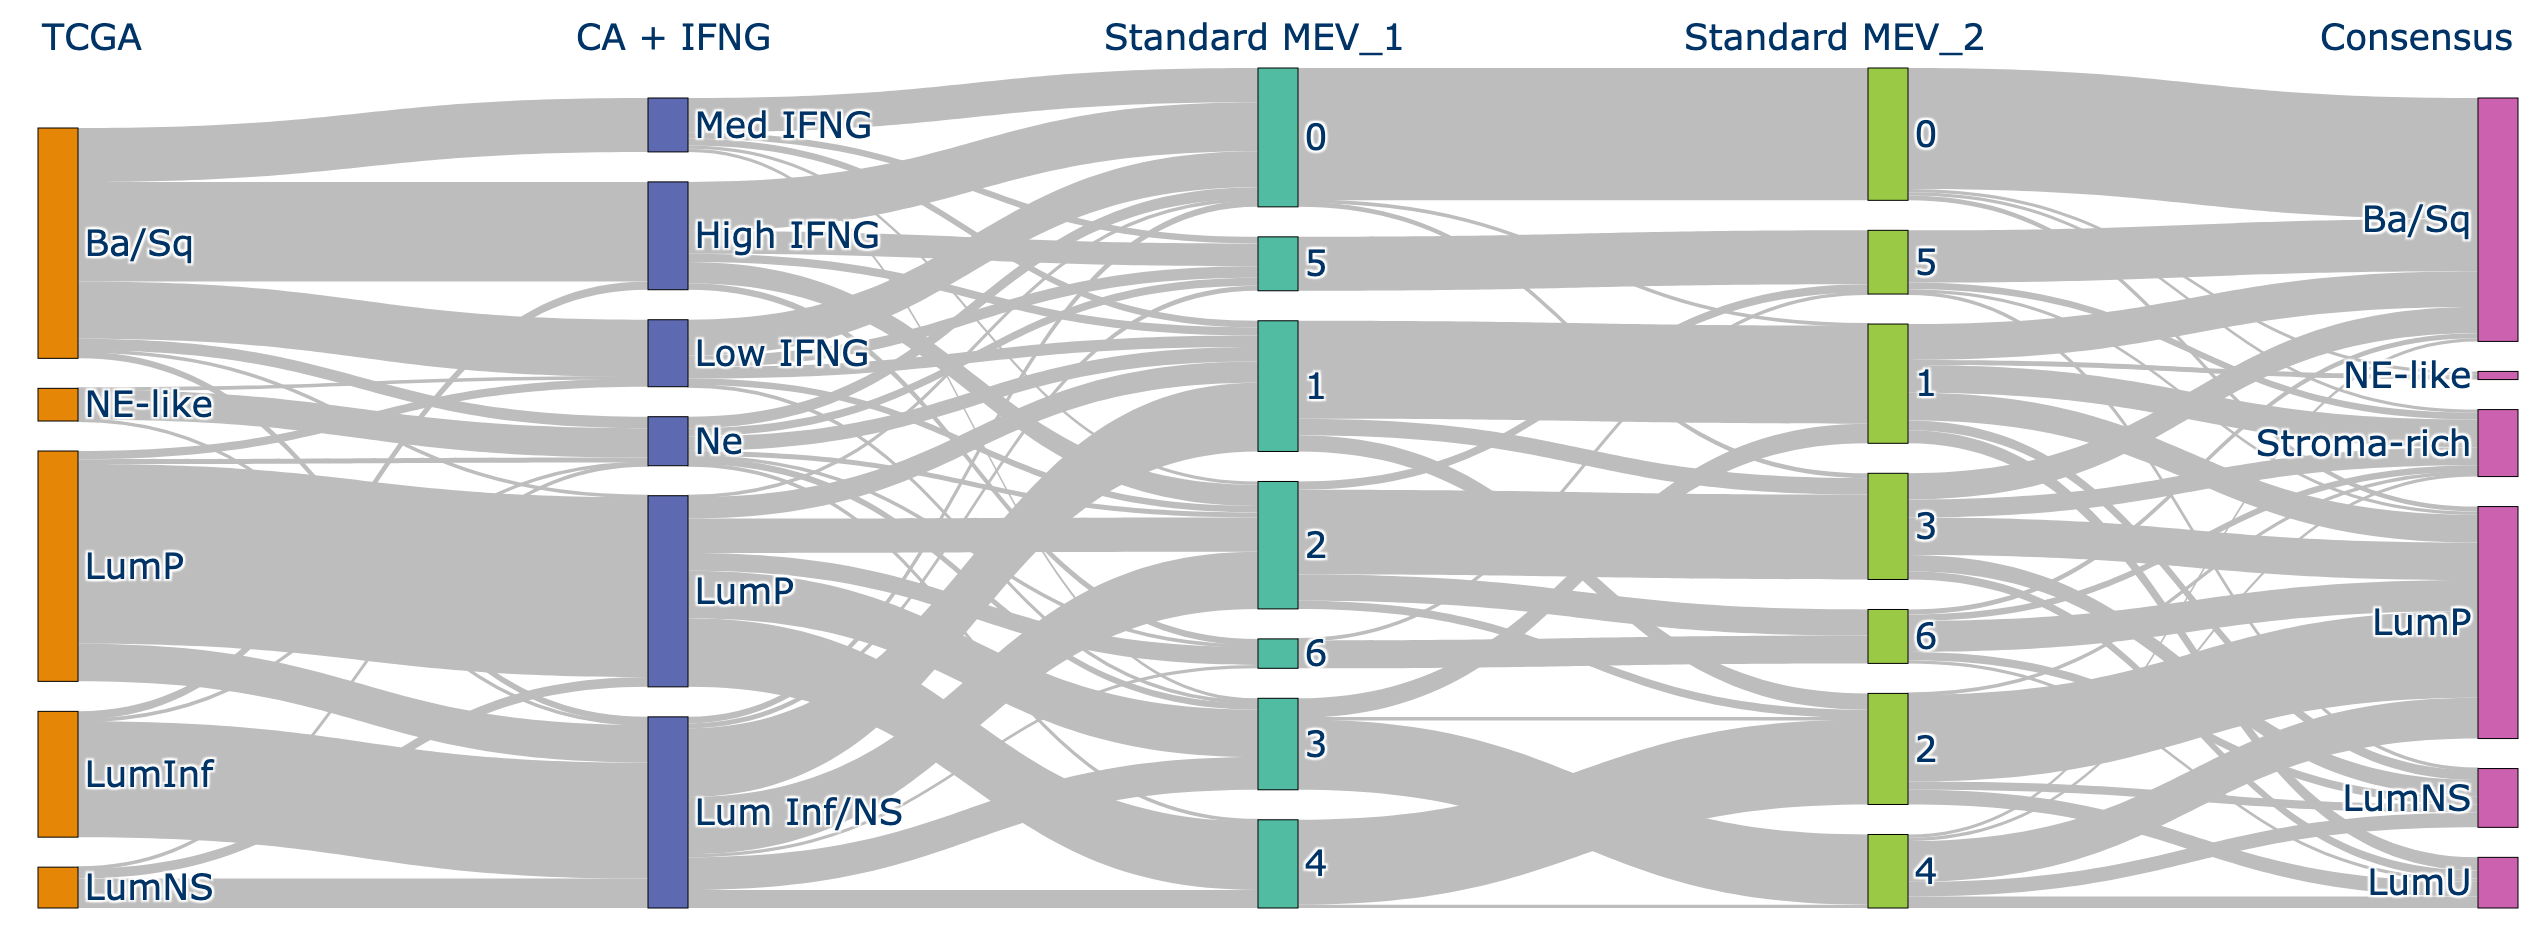
\includegraphics[width=1.0\textwidth,keepaspectratio]{Sections/Network_II/validation/mevs_comp_std_K_7.png}
        \caption{Standard networks}
    \end{subfigure} %
    \centering
    \begin{subfigure}{0.9\linewidth}
        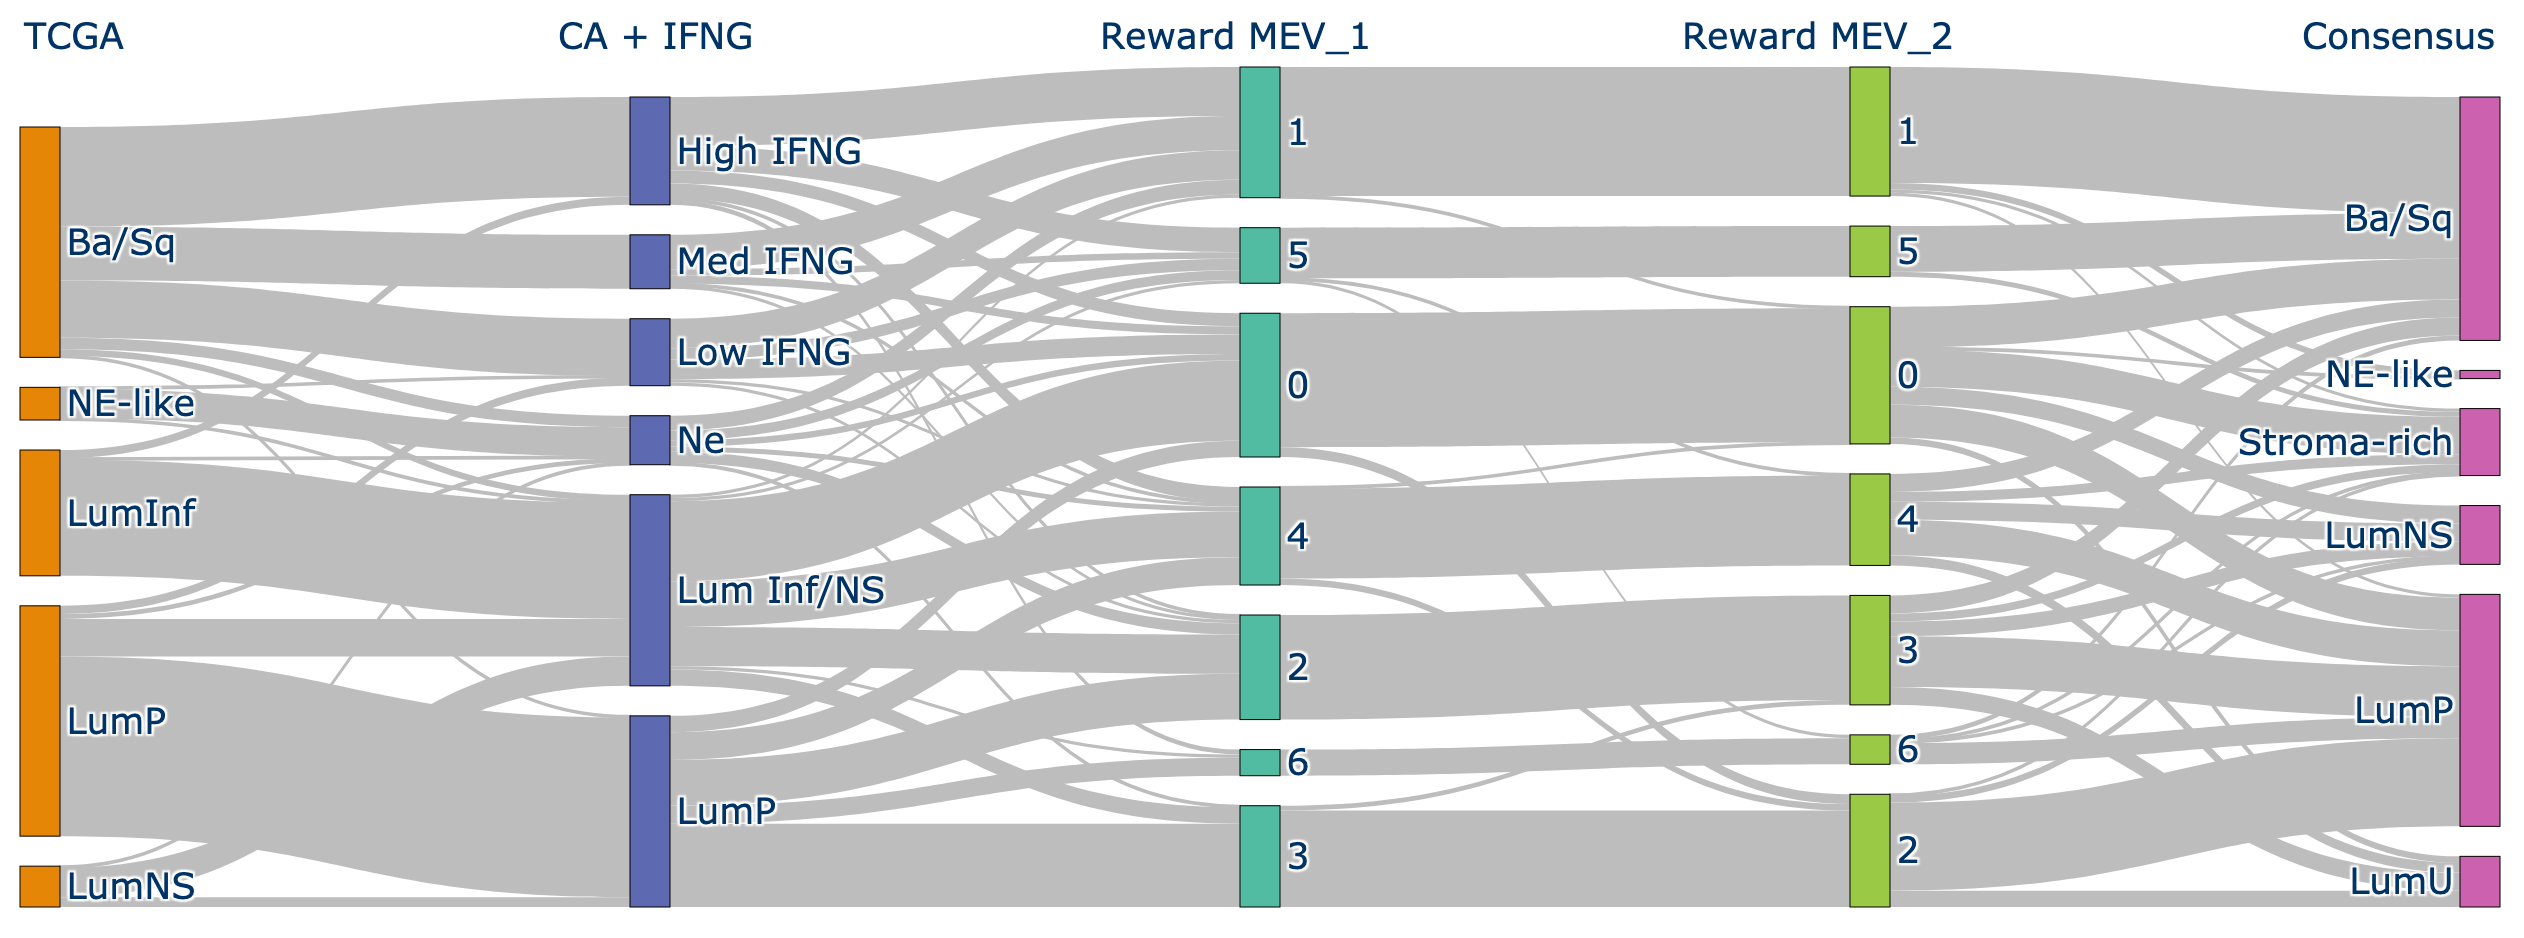
\includegraphics[width=1.0\textwidth,keepaspectratio]{Sections/Network_II/validation/mevs_comp_rwd_K_7.png}
        \caption{Reward v2 networks}
    \end{subfigure}
    \centering
    \caption[MEV vs iMEV with K-means K=5]{In the two subfigures, sankey comparison between TCGA classification \citep{Robertson2017-mg}, the previous MIBC stratification derived in this PhD \cref{s:cs:bio_interp}, the two version of MEVs and the consensus \citep{Kamoun2020-tj}. The subtyping based on the two MEVs are the main groups to compare as the version of MEV only considers the gene expression from TCGA cohort while the second it integrates the non-tumour dataset as well; the other classifications are used for reference. Figure that complements work from \cref{s:N_II:mev_comp}. }
    \label{fig:ap:mevs_comp}
\end{figure}


% Standard 
\section{Standard Network} \label{ap:N_II:coms}

% 25
\begin{figure}[H]    
    \centering
    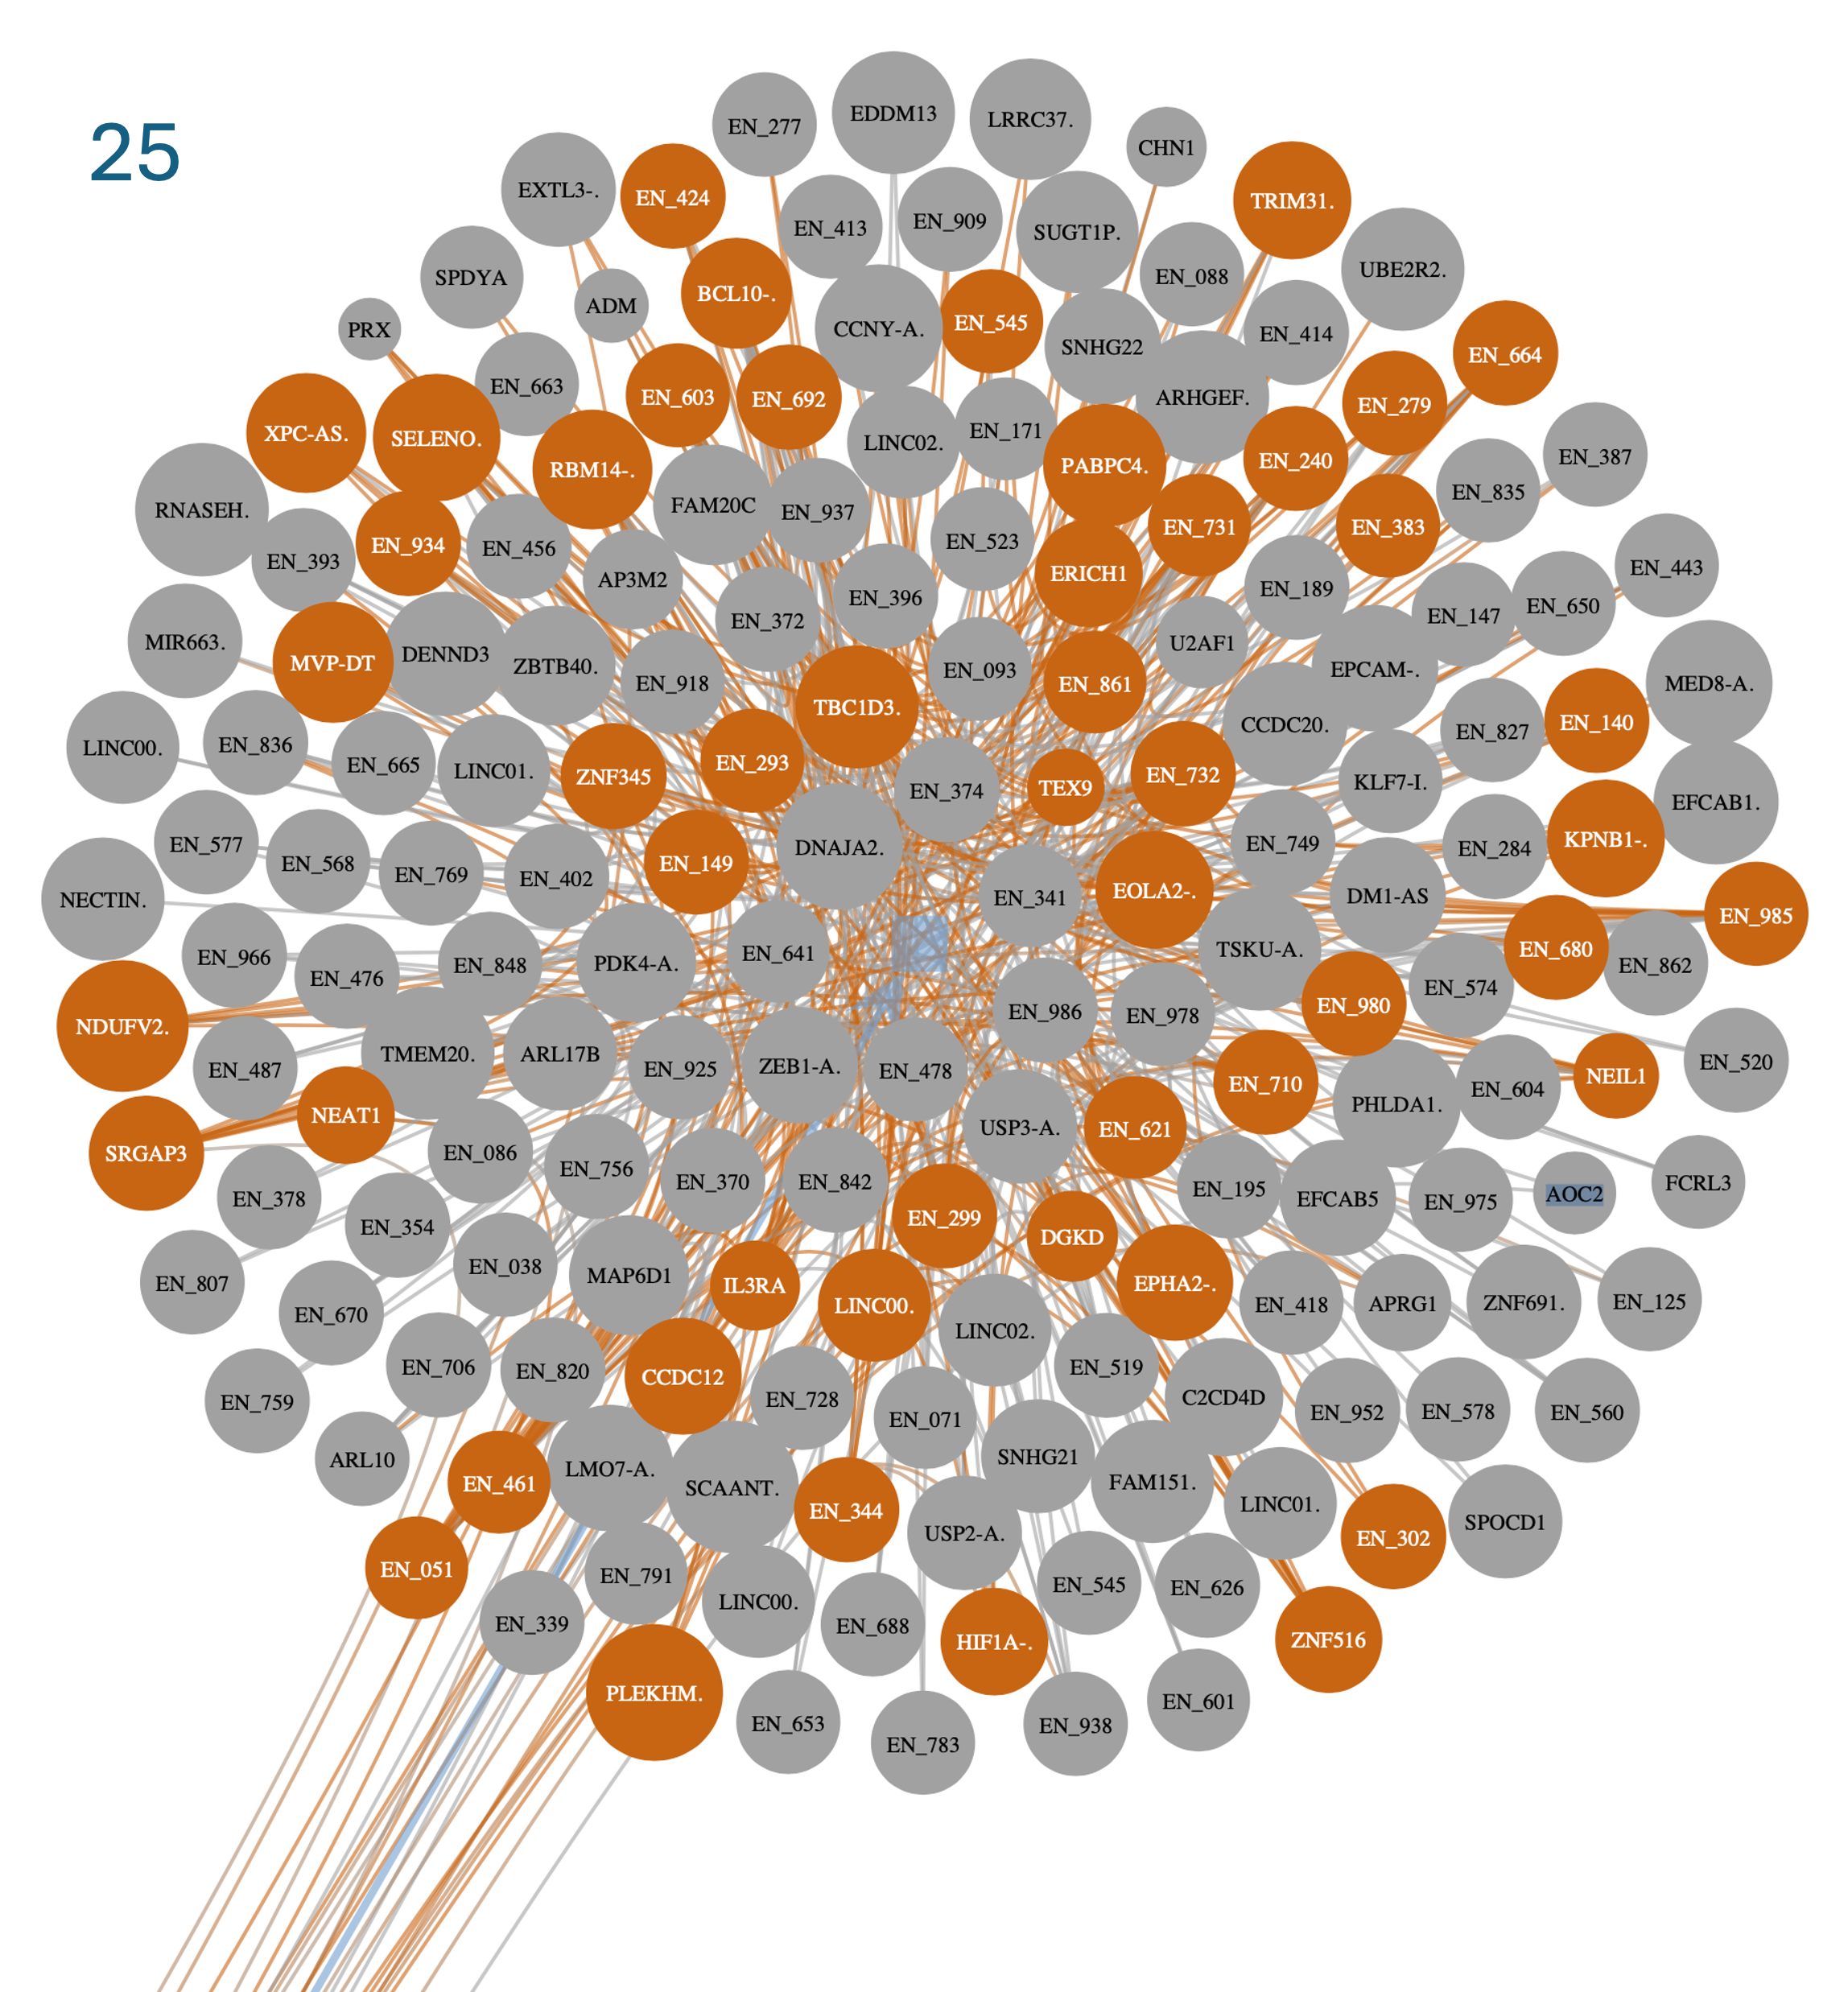
\includegraphics[width=0.9\textwidth,keepaspectratio]{Sections/Network_II/resources/non_tum/25_com.png}
    \caption[Community 25 - driving the healthy and tumour splits]{Community 25 (along with 19 and 29) drives the splits in the tissue differentiation datasets. This community is enriched in the large ABS-Ca and the small P0 subgroups from \cref{fig:N_II:non_tum_sankey_comp}. The community contains 180 genes from which 50 with the highest ModCon score are highlighted in orange. To aid the visualisation some of the genes were trim, for the ones with longer names the first 5 letters were kept while for 'ENSG...' like nodes the "EN\_" and the last 3 digits were kept. See \cref{s:N_II:comm_charact} for more details, community 19 (\cref{fig:N_II:19_com}) and 29 (\cref{fig:ap:com_29}). }
    \label{fig:ap:com_25}
\end{figure}

% 29
\begin{figure}[!htb]    
    \centering
    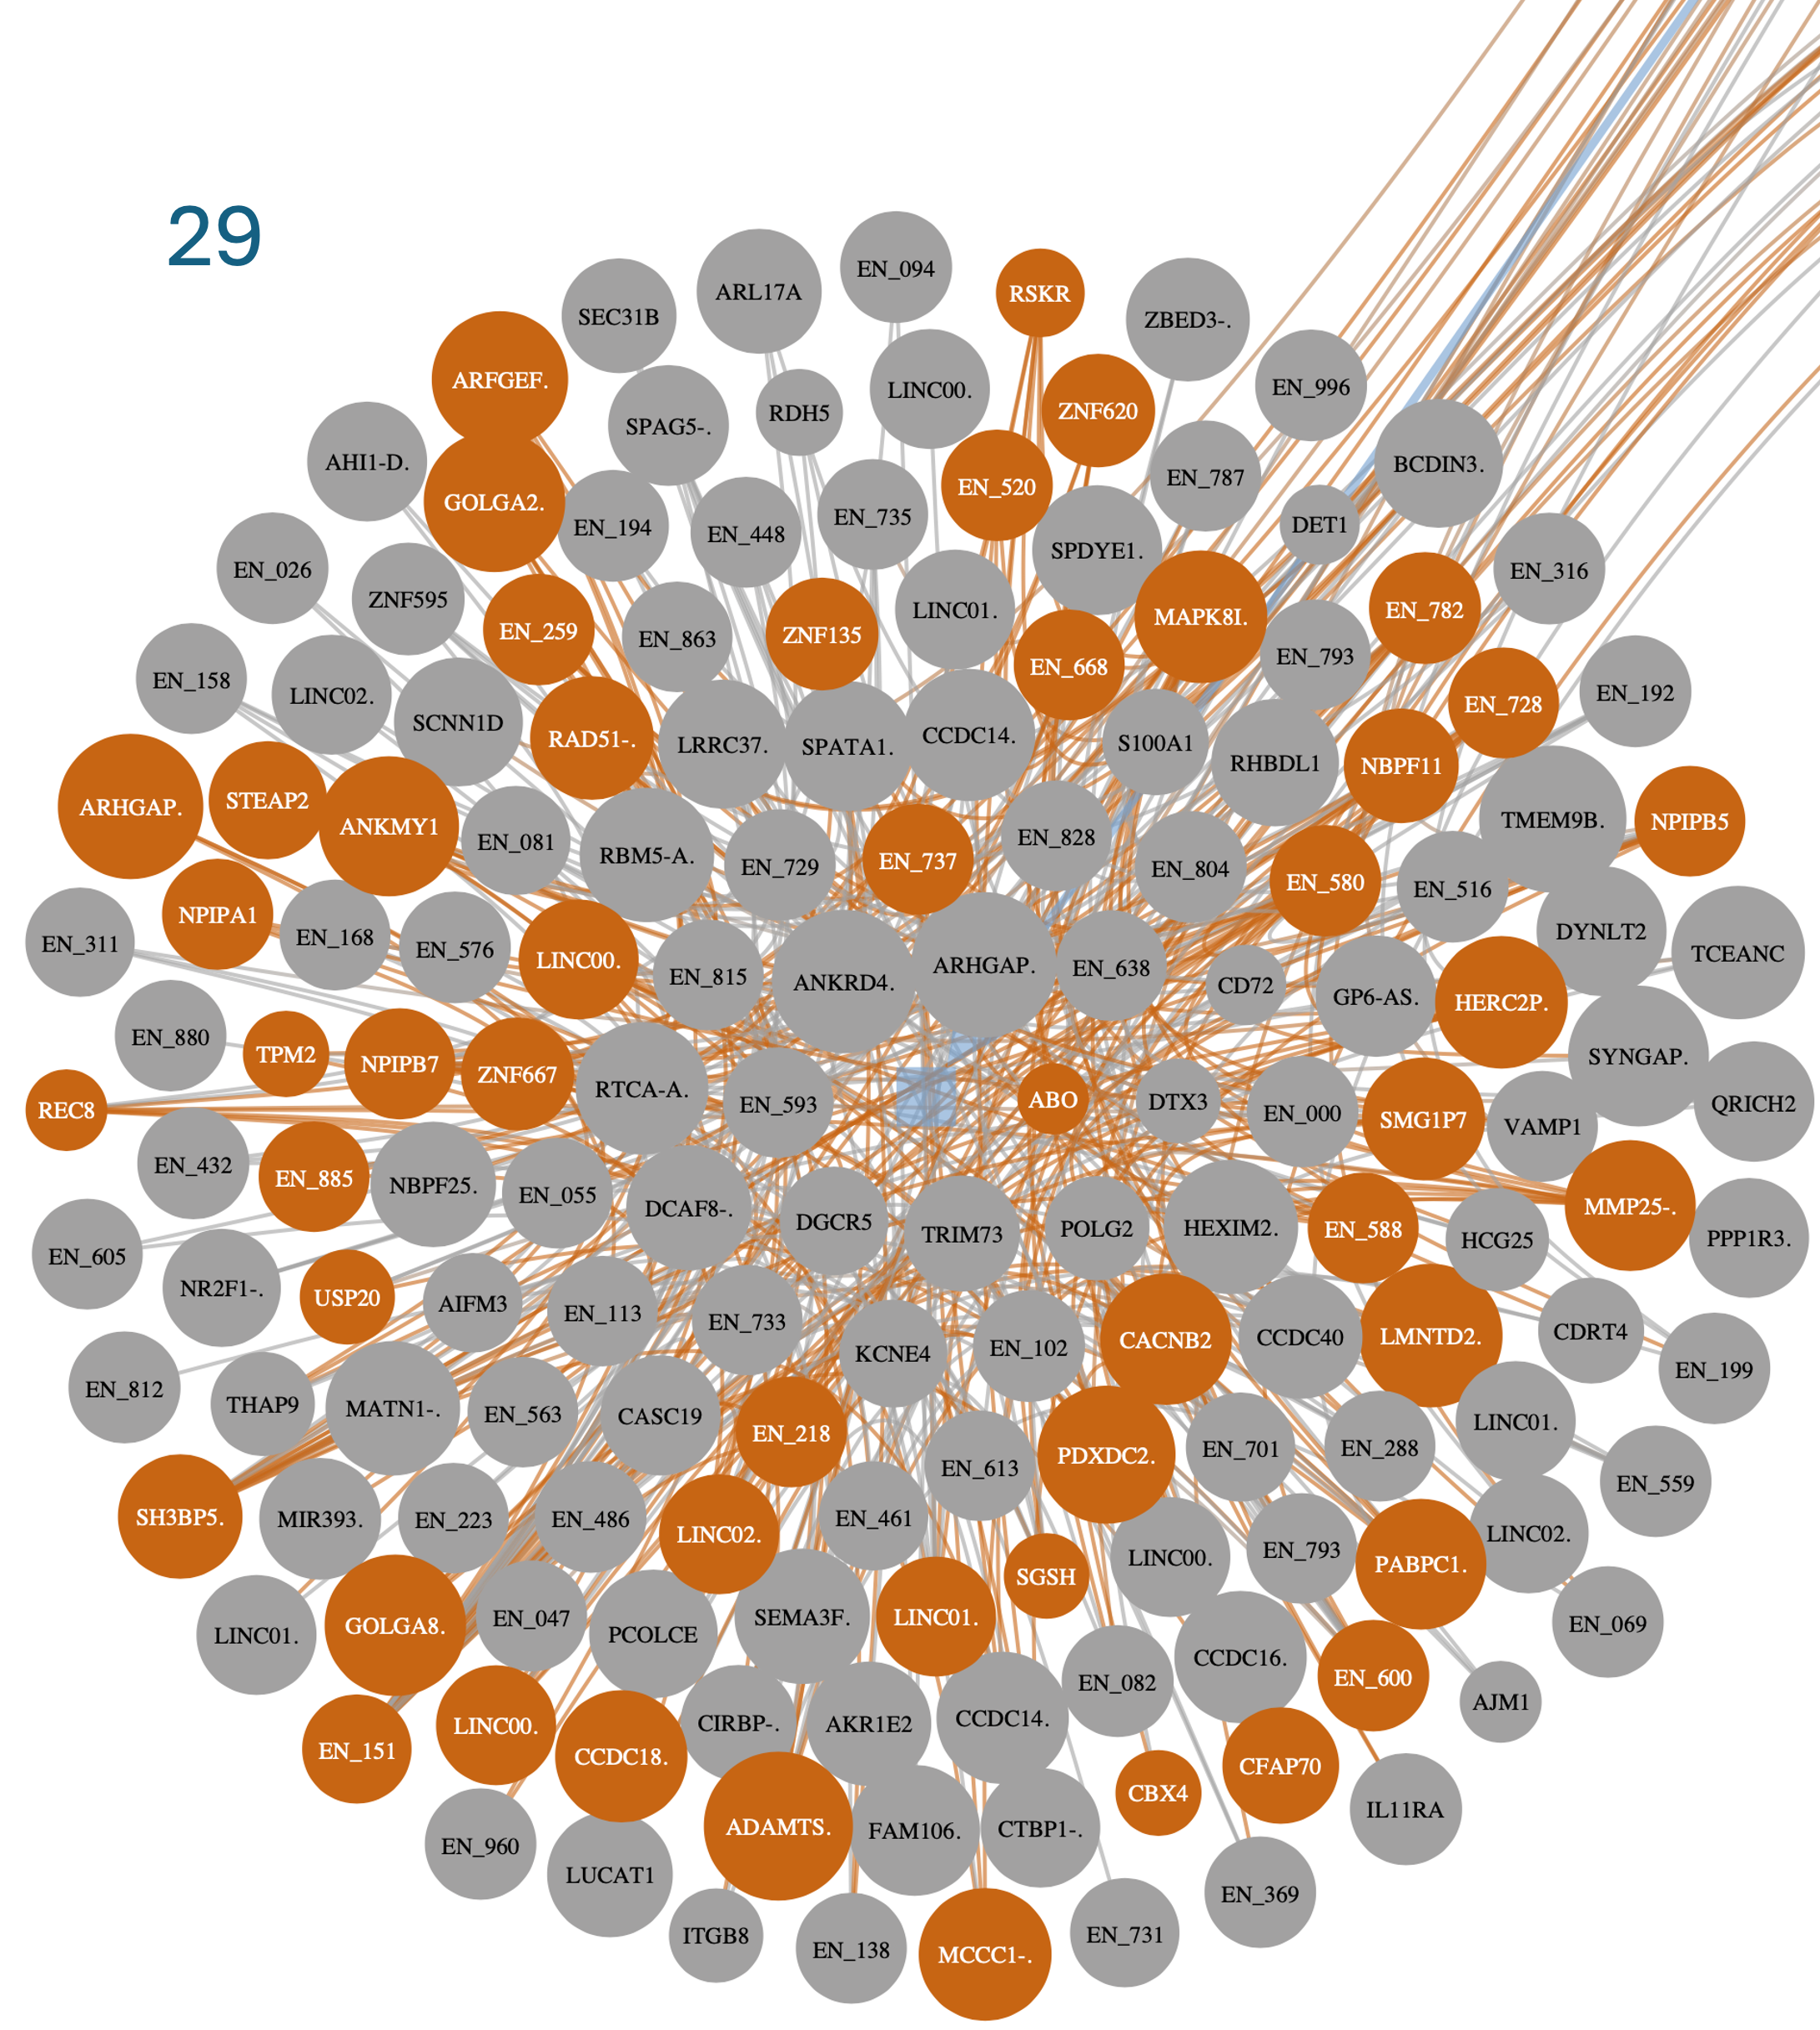
\includegraphics[width=0.9\textwidth,keepaspectratio]{Sections/Network_II/resources/non_tum/29_com.png}
    \caption[Community 29 - driving the healthy and tumour splits]{Community 29 (along with 19 and 25) drives the splits in the tissue differentiation datasets. This community is enriched in the small ABS-Ca and the large P0 subgroups from \cref{fig:N_II:non_tum_sankey_comp}. The community contains 164 genes from which 50 with the highest ModCon score are highlighted in orange. To aid the visualisation some of the genes were trim, for the ones with longer names the first 5 letters were kept while for 'ENSG...' like nodes the "EN\_" and the last 3 digits were kept.  See the network representation of community 19 (\cref{fig:N_II:19_com}) and 29 (\cref{fig:ap:com_29}).}
    \label{fig:ap:com_29}
\end{figure}



% Reward
\section{Reward Network}

% Mean degree 
\begin{sidewaysfigure}   
    \centering
    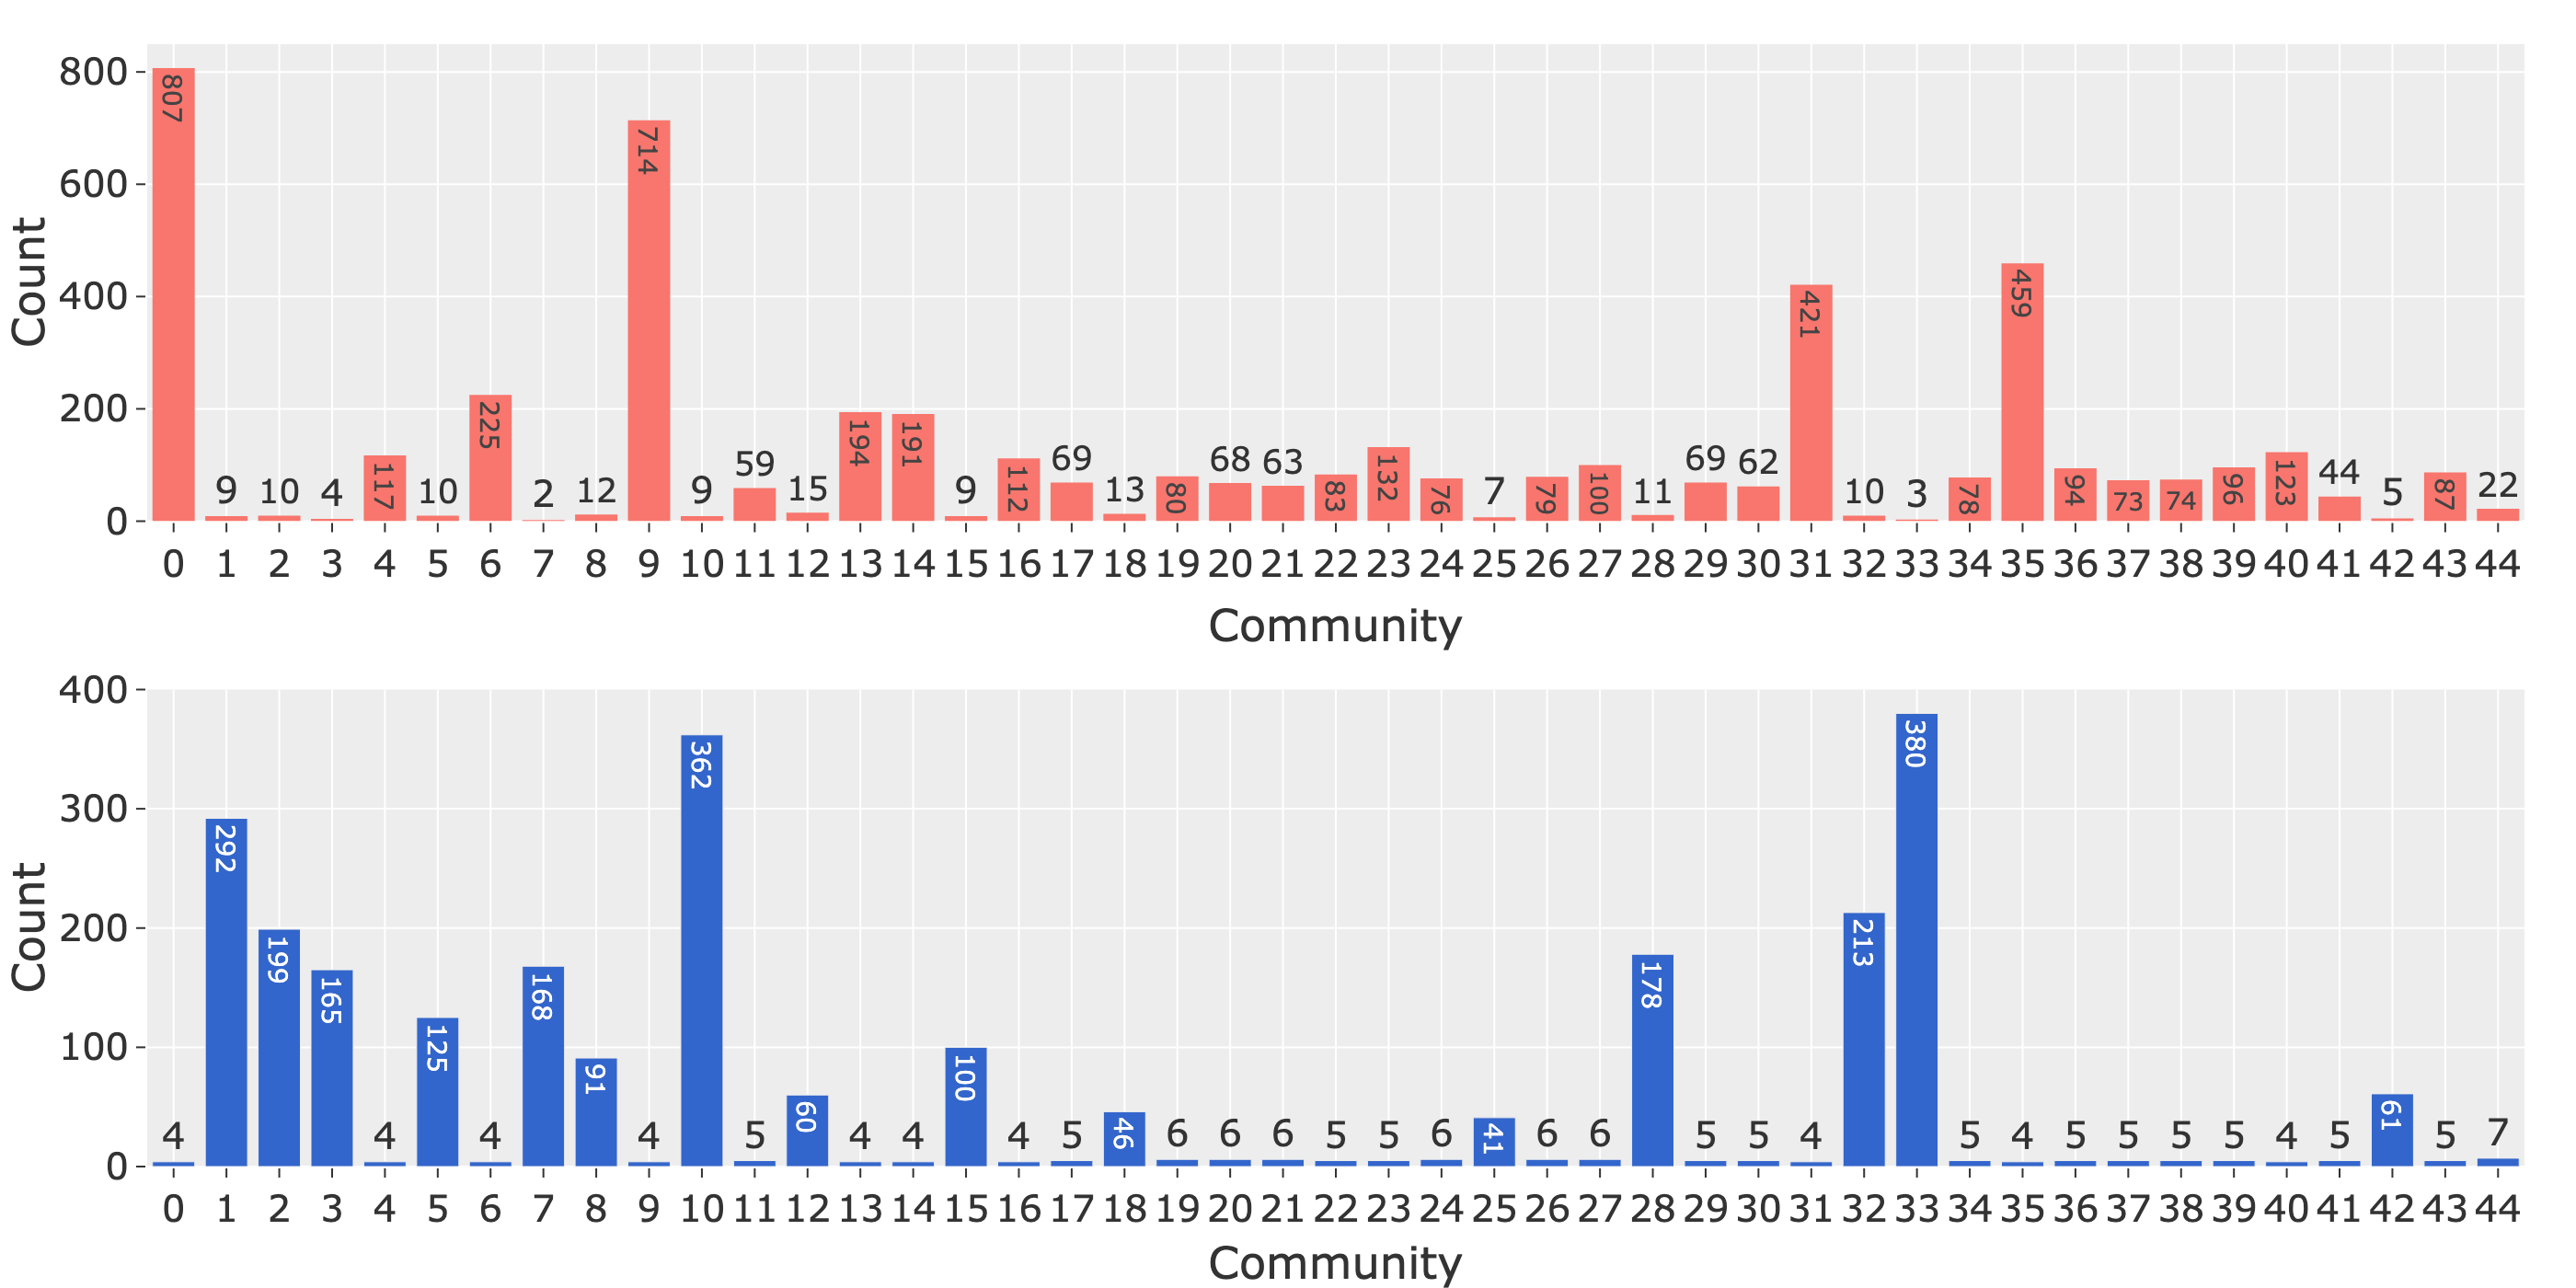
\includegraphics[width=1.0\textwidth,height=1.0\textheight,keepaspectratio]{Sections/Network_II/resources/reward/Degree_vs_ComSize.png}
    \caption[High connected groups: Community size vs Mean degree]{The top bar shows the community size (Y-axis) of the communities while the other plot the mean degree (Y-axis) in a community. This two complementary figures show that communities with a high number of connections are grouped in smaller communities while the large contains nodes with a low node degree. This plot complements the analysis performed in \cref{s:N_II:high_conn}. There is an inverse relationship between the community size and the number of connections.} 
    \label{fig:ap:degree_com_size}
\end{sidewaysfigure}



% High degree communities
\subsection{Network: high degree communities}

The figure below represents the network representation of the small communities (\(<10\) nodes) with a high degree. These genes are explored in more details in \cref{s:N_II:high_conn} and show that are highly and strongly correlated with other genes, and have a high mutation burden. 

\begin{figure}[H]    
    \centering
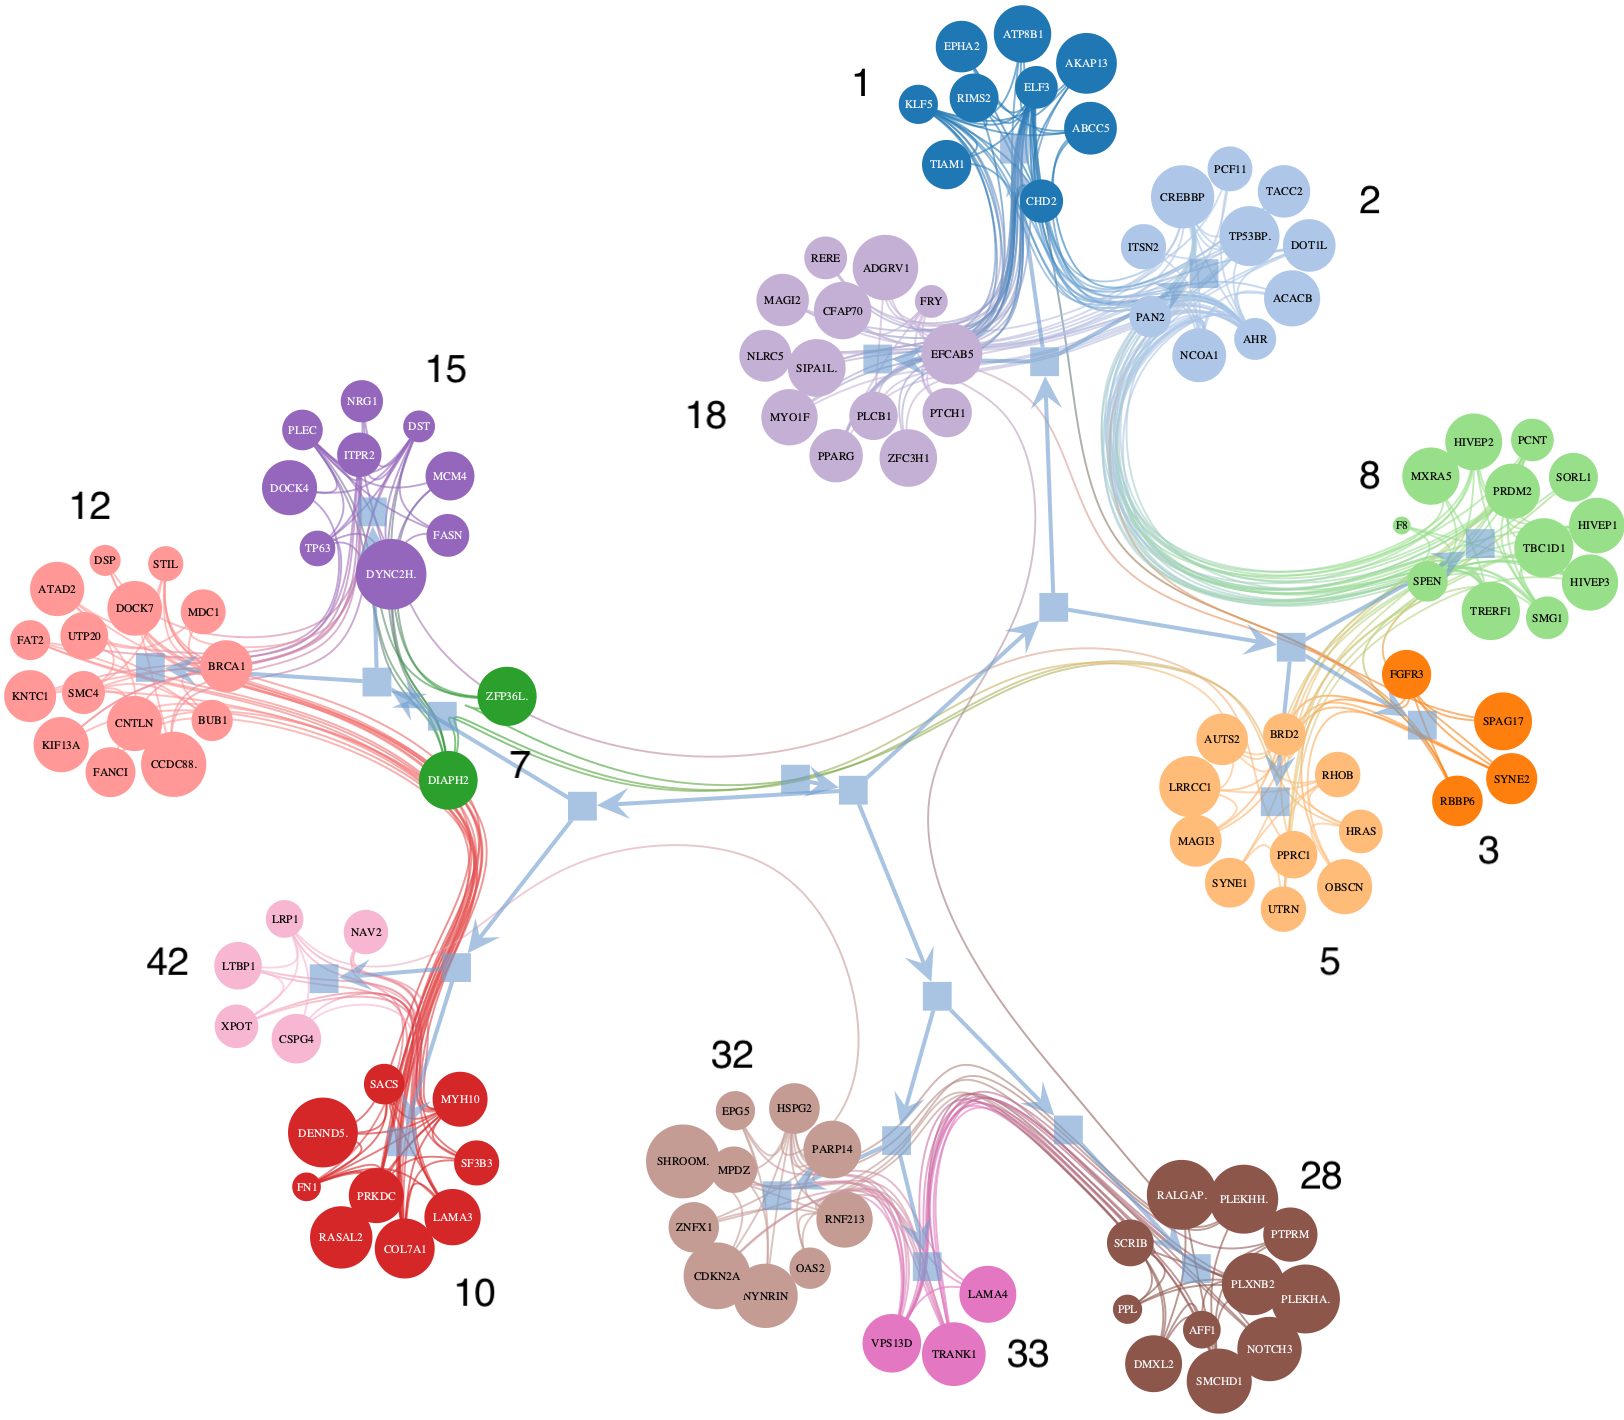
\includegraphics[width=1.0\textwidth,height=1.0\textheight,keepaspectratio]{Sections/Network_II/resources/reward/sel_communities.png}
    \caption[Highly connected communities from the reward network]{Graph representation of the communities that have a high number of connections. There are 14 communities with a total of 122 genes found in the reward network built using the pipeline in \cref{s:N_II:methods}. }
    \label{fig:ap:graph_smallCom}
\end{figure}



% cluster analysis
\subsection{Cluster analysis} \label{s:ap:N_II:clustering analysis}

This section covers the cluster analysis performed on the MEV values derived using second version of the network pipeline covered in \cref{s:N_II:rwd}. The aim here is to find the appropriate the clustering model and its configuration. To achieve this the methods from \cref{s:cs:methods} are used which includes the clustering metrics covered in \cref{s:lit:clustering_metrics} and shown in \cref{fig:ap:n_II:cluster_metrics} as well as the Sankey comparison plot in \cref{fig:ap:cs_sankey}.

% Presetn the figure
The three metrics used to measure the performance of the clustering models are Silhouete with cosine distance, Calinski Habrasz and Davies Bouldin. For $K\in[2,14]$ five different clustering metrics were used: K-Means, Ward, Birch, Gaussian Mixture and Spectral Clustering. The average metric values across the clustering models and configurations are plotted in \cref{fig:ap:n_II:cluster_metrics}. The X across the bar signals the overall ranking across the models: rank 1 - X, rank 2 - XX, rank 3 - XXX.


The metrics trends are similar to what is observed in previous clustering analyses (\cref{fig:cs:cs_metrics,fig:ap:non_pca_metrics}), where the models' performance decreases proportionally with the number of groups. This trend is most visible in \cref{fig:ap:n_II:cal_hab} and \cref{fig:ap:n_II:dav_boul}. It can also be noted that the average Silhouette values are below the 'well-clustered' threshold of 0.5 and are lower compared to the clustering performed on the PCA-applied expression data in \cref{fig:cs:cs_metrics}. As indicated by the 'X' markers, the top-performing models are K-Means, Ward, and Spectral Clustering across all three metrics. The models configured to find 4 groups seem to perform the best, which can be explained by the fact that this is closest to $K=2,3$, which have the highest scoring values; this has been discussed in more detail in the cluster analysis from \cref{s:clustering_analysis}.

% Top table
The top metrics from \cref{fig:ap:n_II:cluster_metrics} are extracted in the table \cref{tab:ap:N:II:top_3_cs} which clearly shows that $K=4$ is the preferred number of groups with Spectral, K-means and Ward. The comparison of the MIBC stratification in \cref{fig:ap:cs_sankey} shows the three clustering models compared with TCGA, consensus and the subtypes derived in the first chapter of thesis \cref{s:cs:bio_interp}. Across all the models there is no basal split which can be explained by the low K. It can be noticed that Spectral Clustering and Ward have a higher imbalance across the group sizes compared with K-means. The first model having the 0 group which holds most of the luminal samples (TCGA/consensus), while the latter is having a 0 group which contains the Basal Squamous samples and some of the LumP (consensus). For the more balanced size of groups the K-means is preferred over the models.

\begin{figure}[H]
    \captionsetup[subfigure]{justification=Centering}
    \centering
    \begin{subfigure}[!t]{1.0\textwidth}
        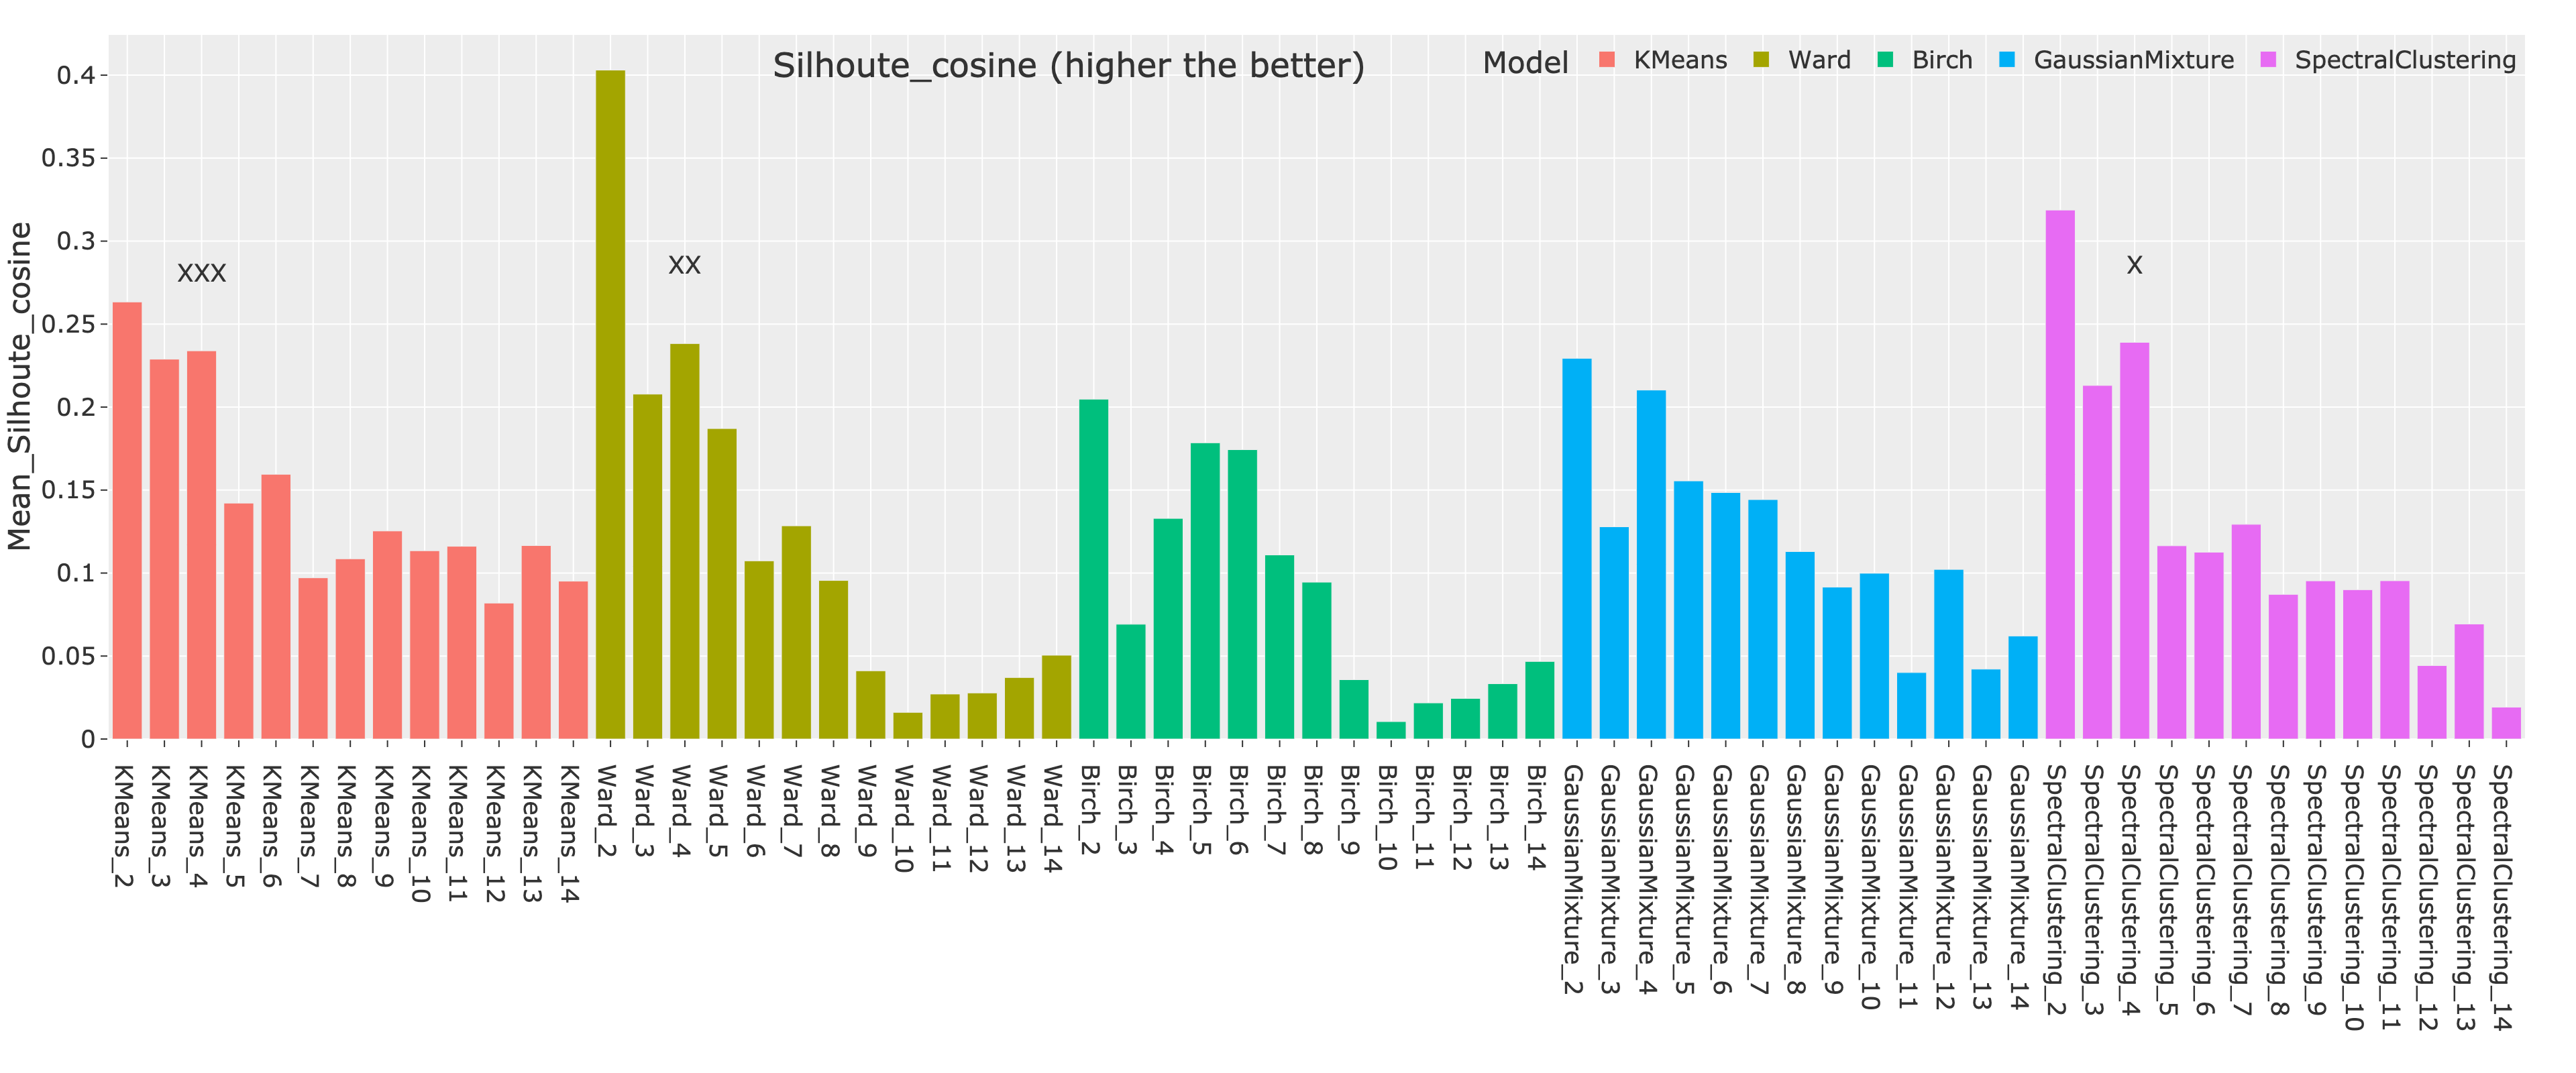
\includegraphics[width=\textwidth]{Sections/Network_II/resources/reward/cluster_analysis/allComs_top3_Silhoute_cosine.png}
        \caption{Silhouette using cosine distance}
        \label{fig:ap:n_II:cosine}
    \end{subfigure}
    \centering
    \begin{subfigure}[!t]{1.0\textwidth}
        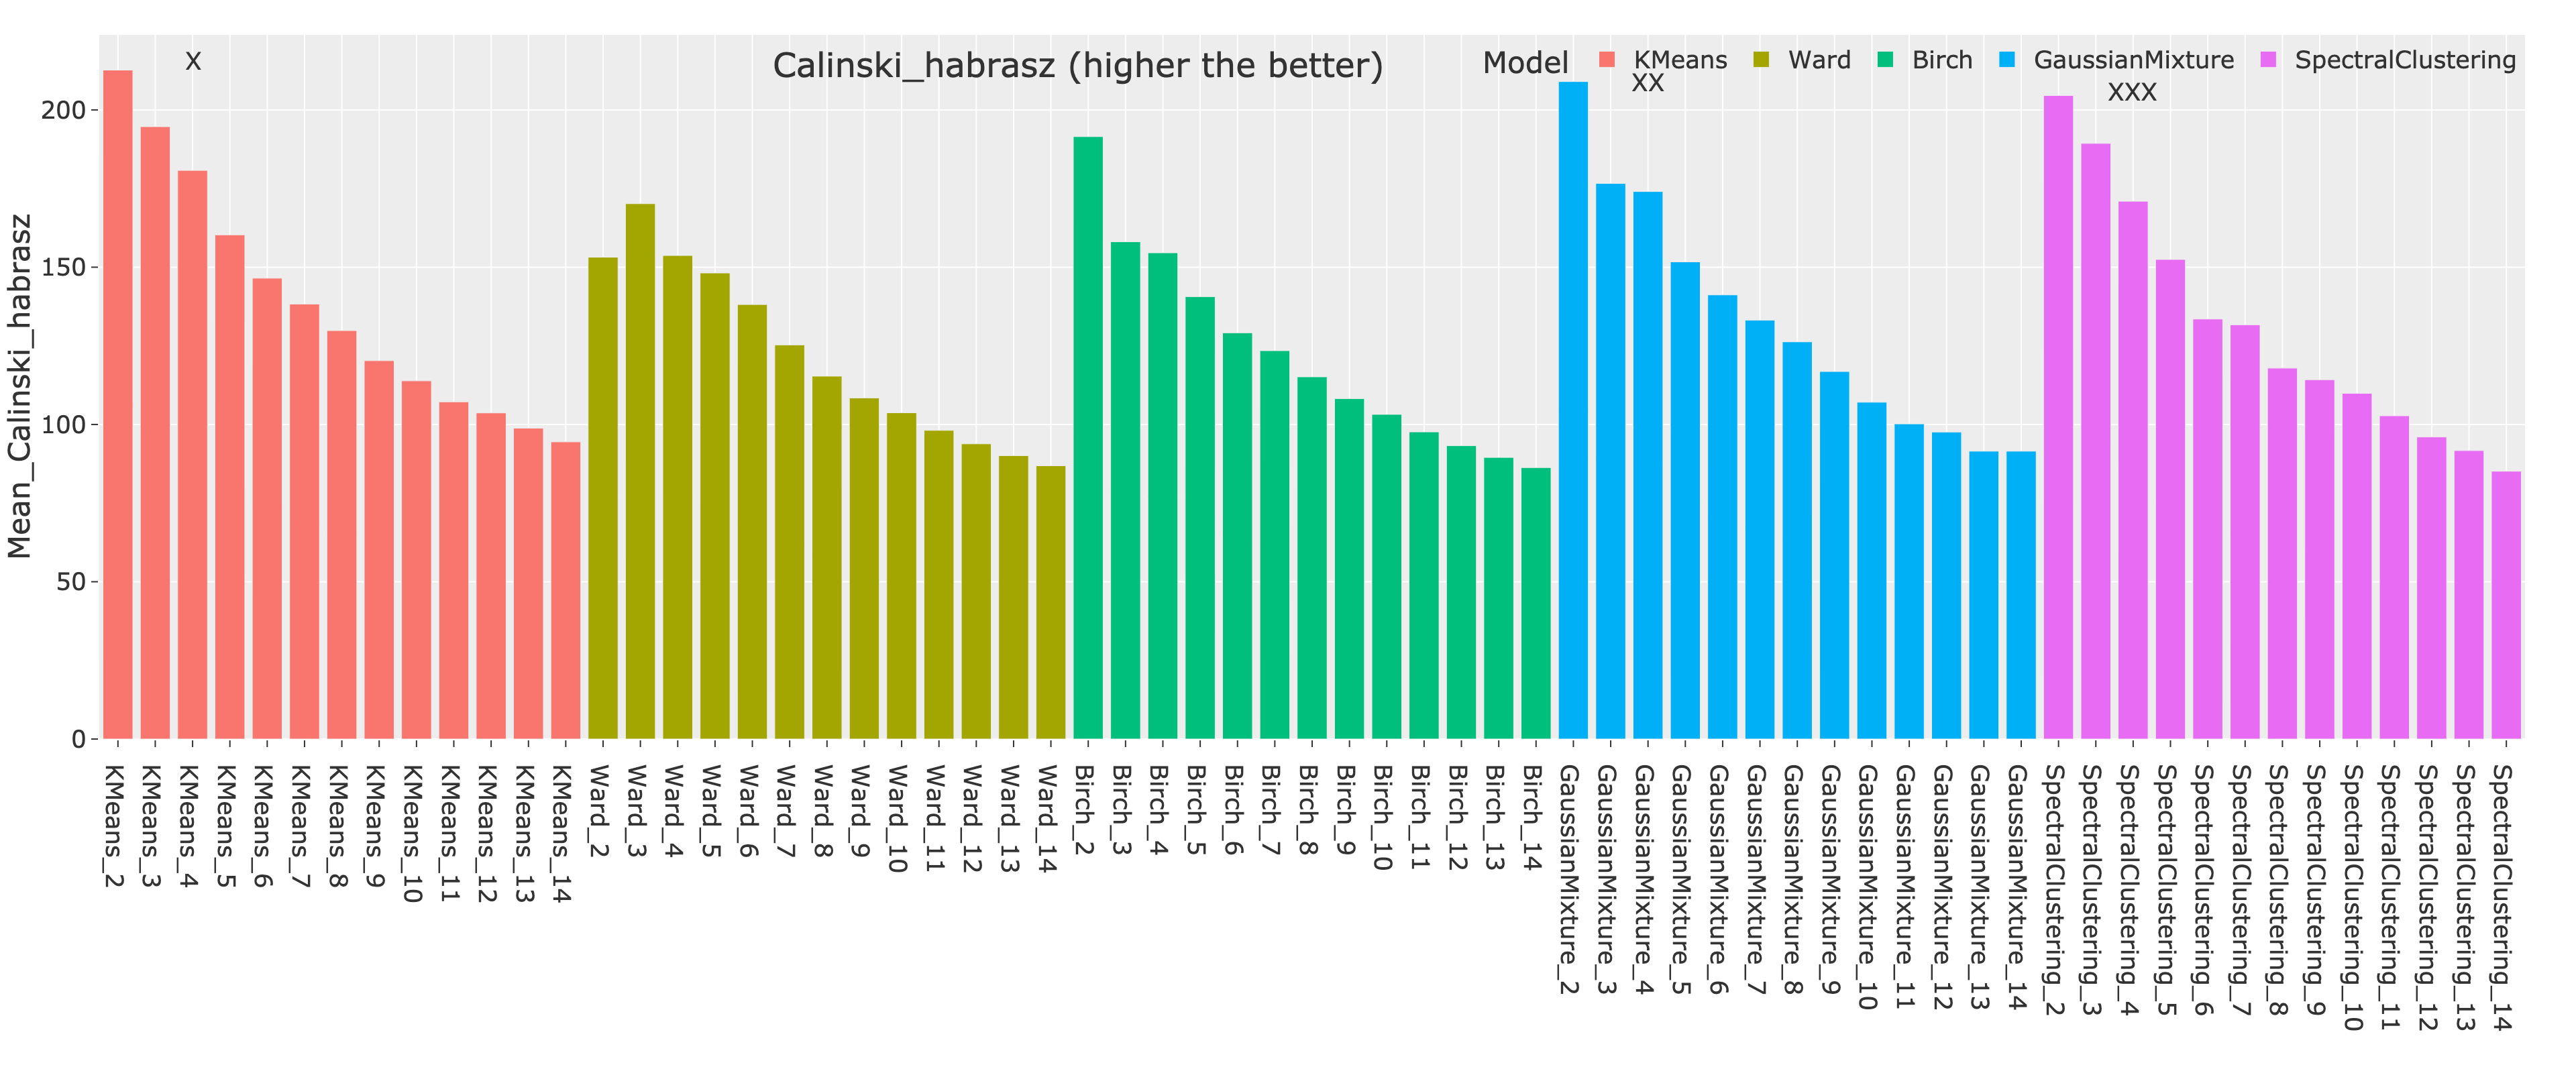
\includegraphics[width=\textwidth]{Sections/Network_II/resources/reward/cluster_analysis/allComs_top3_Calinski_habrasz.png}
        \caption{Calinski Harabasz}
        \label{fig:ap:n_II:cal_hab}
    \end{subfigure}
    \centering
    \begin{subfigure}[!t]{1.0\textwidth}
        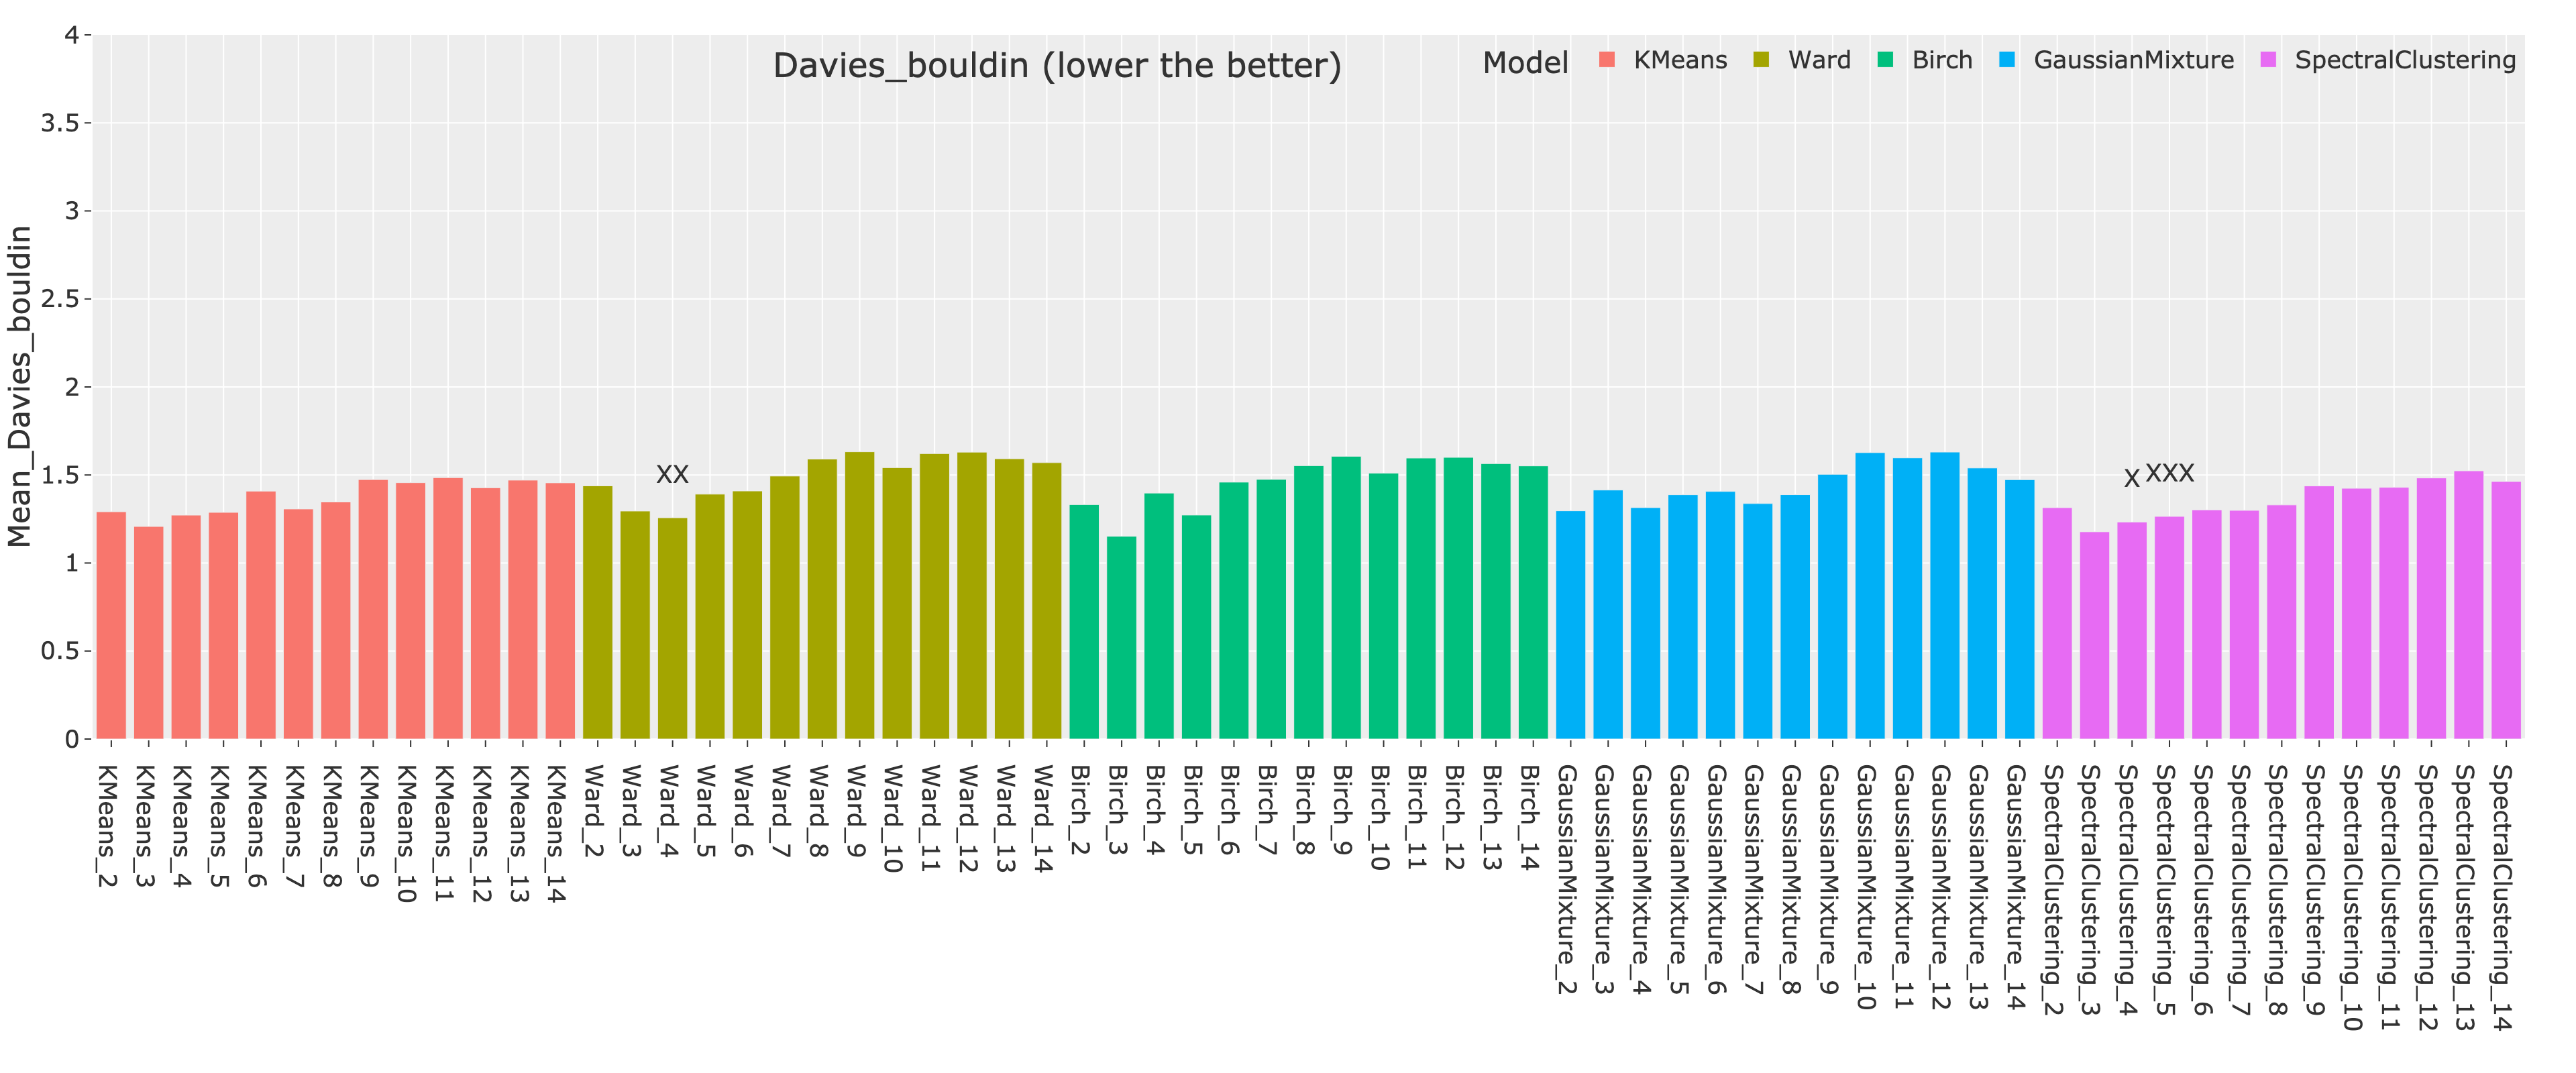
\includegraphics[width=\textwidth]{Sections/Network_II/resources/reward/cluster_analysis/allComs_top3_Davies_bouldin.png}
        \caption{Davies Bouldin}
        \label{fig:ap:n_II:dav_boul}
    \end{subfigure}
    \caption[Clustering analysis for the healthy reward network]{The means of the two cluster metrics introduced in \cref{s:lit:clustering_metrics}: Silhouette (cosine), Calinski Harabasz and Davies Bouldin. Each of them assess different aspects of clustering and are used to determine the right clustering model for the MIBC cohort from TCGA. The X across the bar signals the overall ranking across the models: rank 1 - X, rank 2 - XX, rank 3 - XXX. The clusters are derived from using the MEVs for the reward network derived in \cref{s:N_II:rwd}.}
    \label{fig:ap:n_II:cluster_metrics}
\end{figure}


\begin{table}[h!]
    \centering
    \begin{tabular}{|p{6cm}|p{6cm}|}
        \hline
        \textbf{Metric} & \textbf{Cluster model} \\
        \hline
        \#1 Silhouette cosine & \rule{0pt}{2.5ex} Spectral 4 \\
        \hline
        \#2 Silhouette cosine & \rule{0pt}{2.5ex} Ward 4 \\
        \hline
        \#3 Silhouette cosine & \rule{0pt}{2.5ex} K-means 4 \\
        \hline
        \#1 Calinski Habrasz & \rule{0pt}{2.5ex} K-means 4 \\
        \hline
        \#2 Calinski Habrasz & \rule{0pt}{2.5ex} Gaussian Mixture 4 \\
        \hline
        \#3 Calinski Habrasz & \rule{0pt}{2.5ex} Spectral 4 \\
        \hline
        \#1 Davies Bouldin & \rule{0pt}{2.5ex} Spectral 4 \\
        \hline
        \#2 Davies Bouldin & \rule{0pt}{2.5ex} Ward 4 \\
        \hline
        \#3 Davies Bouldin & \rule{0pt}{2.5ex} Spectral 5 \\
        \hline
    \end{tabular}
    \caption[Top performing clustering model]{Top three clustering models and their configuration based on the three metrics Silhouette cosine, Calinski Habrasz, and Davies Bouldin. This table is a summary of the pointed configurations in \cref{fig:ap:n_II:cluster_metrics}.}
    \label{tab:ap:N:II:top_3_cs}
\end{table}

% Sankey - highlight the imbalance in the groups
Due to the trends in the metrics decreasing proportionally with the number of groups, further analysis is needed to decide on the optimal value of $K$. For this purpose, K-means clustering with $K \in [2,14]$ was performed, and the number of samples with negative Silhouette values was counted. These subsets of samples represent those which were incorrectly grouped, providing additional information on the clustering performance. The results are plotted in a bar chart in \cref{fig:ap:neg_samples}, where the Y-axis represents the number of negative samples and the X-axis represents the value of $K$ used in K-means clustering.

% Using the negative samples to decide
In \cref{fig:ap:neg_samples}, the same trend as before can be observed, where performance decreases proportionally with increasing $K$. The best clustering model is when $K=2$, followed by $K=5$ and $K=7$, indicating that these group sizes are the most appropriate for the clustering model. 


Based on the survival analysis, $K=7$ is chosen as the additional two groups provide higher resolution with minimal negative impact. This is clearly seen in the Kaplan-Meier survival plots for $K=5$ in \cref{fig:ap:survival_K_5} and $K=7$ in \cref{fig:N_II:survival_K_7}. In the first plot, two survival trends are evident, corresponding to the two main groups, large and luminal. In the second figure, when $K=7$, additional aggressive groups are identified.

Overall, the cluster analysis demonstrates the heterogeneity of the disease by not having clearly separated clusters. It is worth mentioning that hierarchical clustering within the Morpheus software \cite{Broad-Institute2016-tn} was explored as an alternative (based on the work from \cref{s:N_II:std}), but the MIBC group sizes were greatly imbalanced.

\begin{figure}[H]    
    \centering
    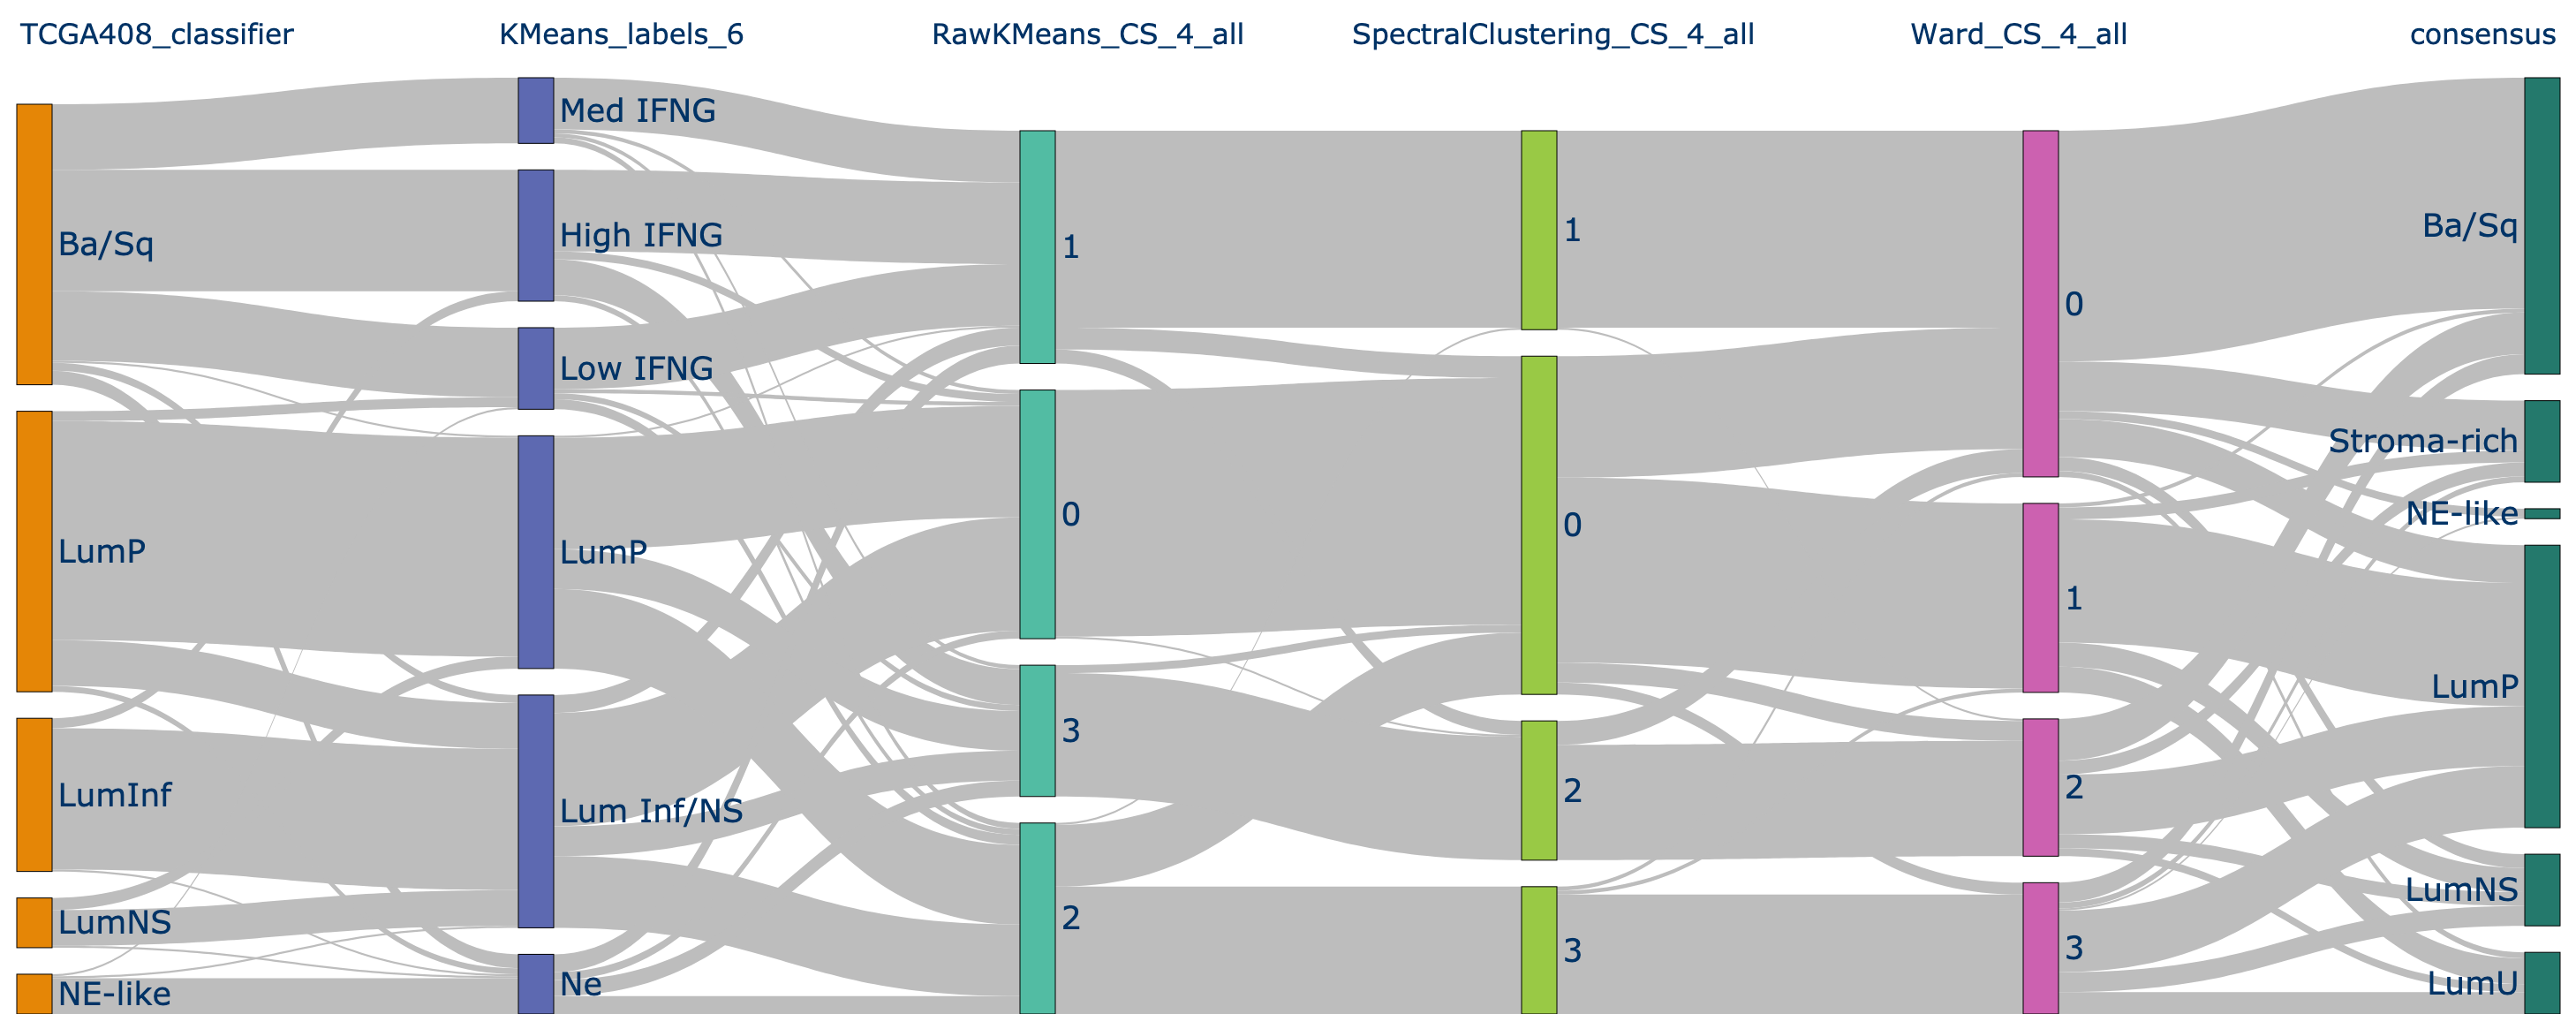
\includegraphics[width=1.0\textwidth,height=1.0\textheight,keepaspectratio]{Sections/Network_II/resources/reward/cluster_analysis/cluster_comp.png}
    \caption[MIBC subtypes comparisons across clustering models]{Comparison between the best performing clustering models and configurations from \cref{fig:ap:n_II:cluster_metrics}: K-Means, Spectral Clustering, and Ward with $K=4$. These models are compared with the classifications from TCGA \citep{Robertson2017-mg}, the consensus \citep{Kamoun2020-tj}, and the previous subtypes derived in the first part of the thesis \cref{s:cs:methods}.}
    \label{fig:ap:cs_sankey}
\end{figure}

\begin{figure}[H]    
    \centering
    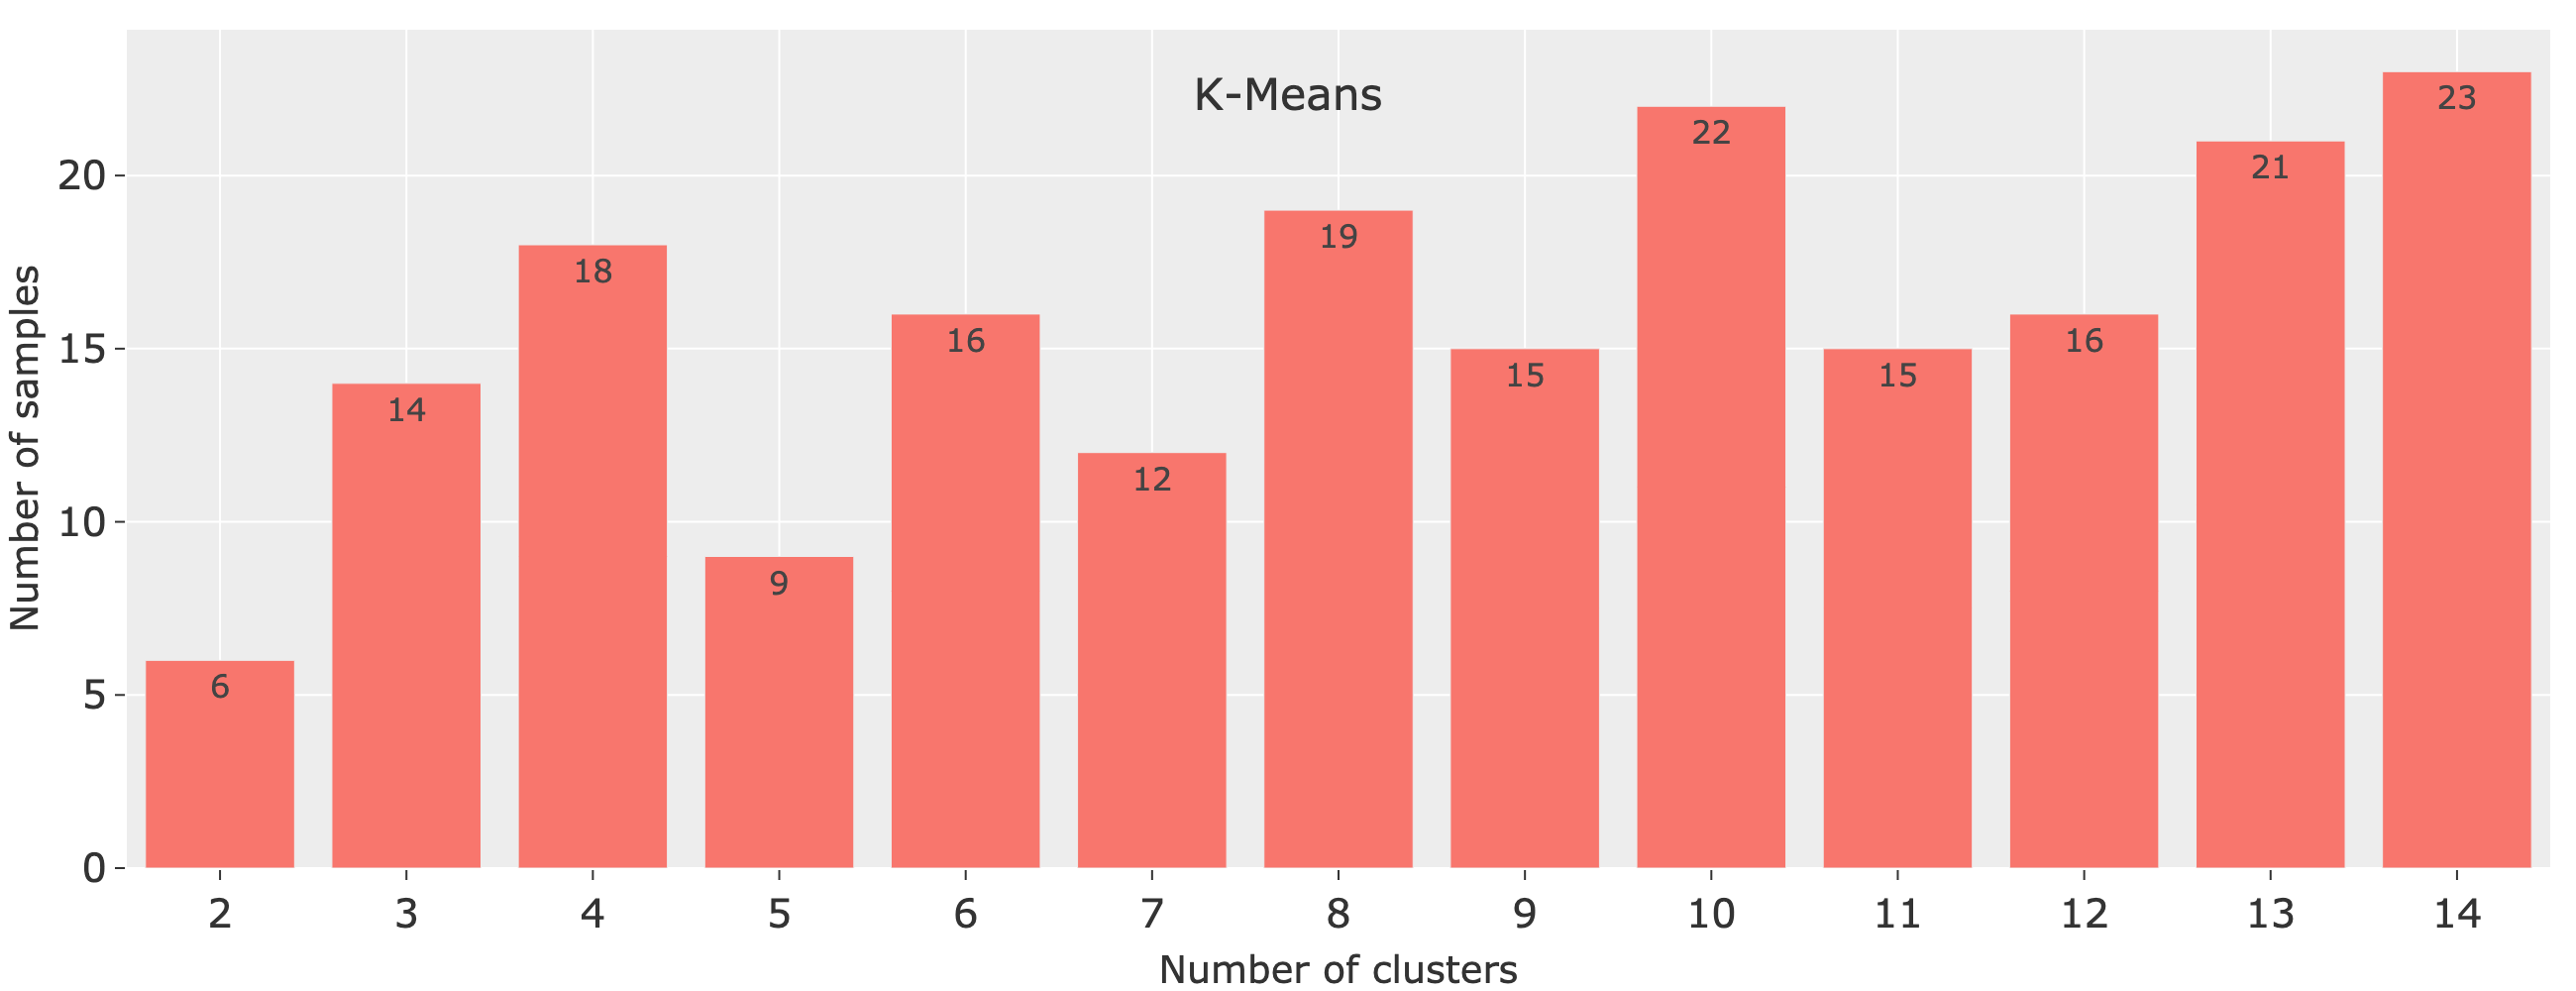
\includegraphics[width=1.0\textwidth,height=1.0\textheight,keepaspectratio]{Sections/Network_II/resources/reward/cluster_analysis/neg_samples.png}
    \caption[Negative silhouette samples]{Negative samples of K-means with $K \in [2,14]$ determined using silhouette cosine. The Y-axis represents the number of samples, while the X-axis represents the number of groups set in the clustering model. As expected, the fewest negative samples occur when $K=2$, and these increase proportionally with $K$. When K-means is configured to find 5 and 7 groups, these configurations have the next lowest number of negative silhouette samples.}
    \label{fig:ap:neg_samples}
\end{figure}

\begin{figure}[H]    
    \centering
    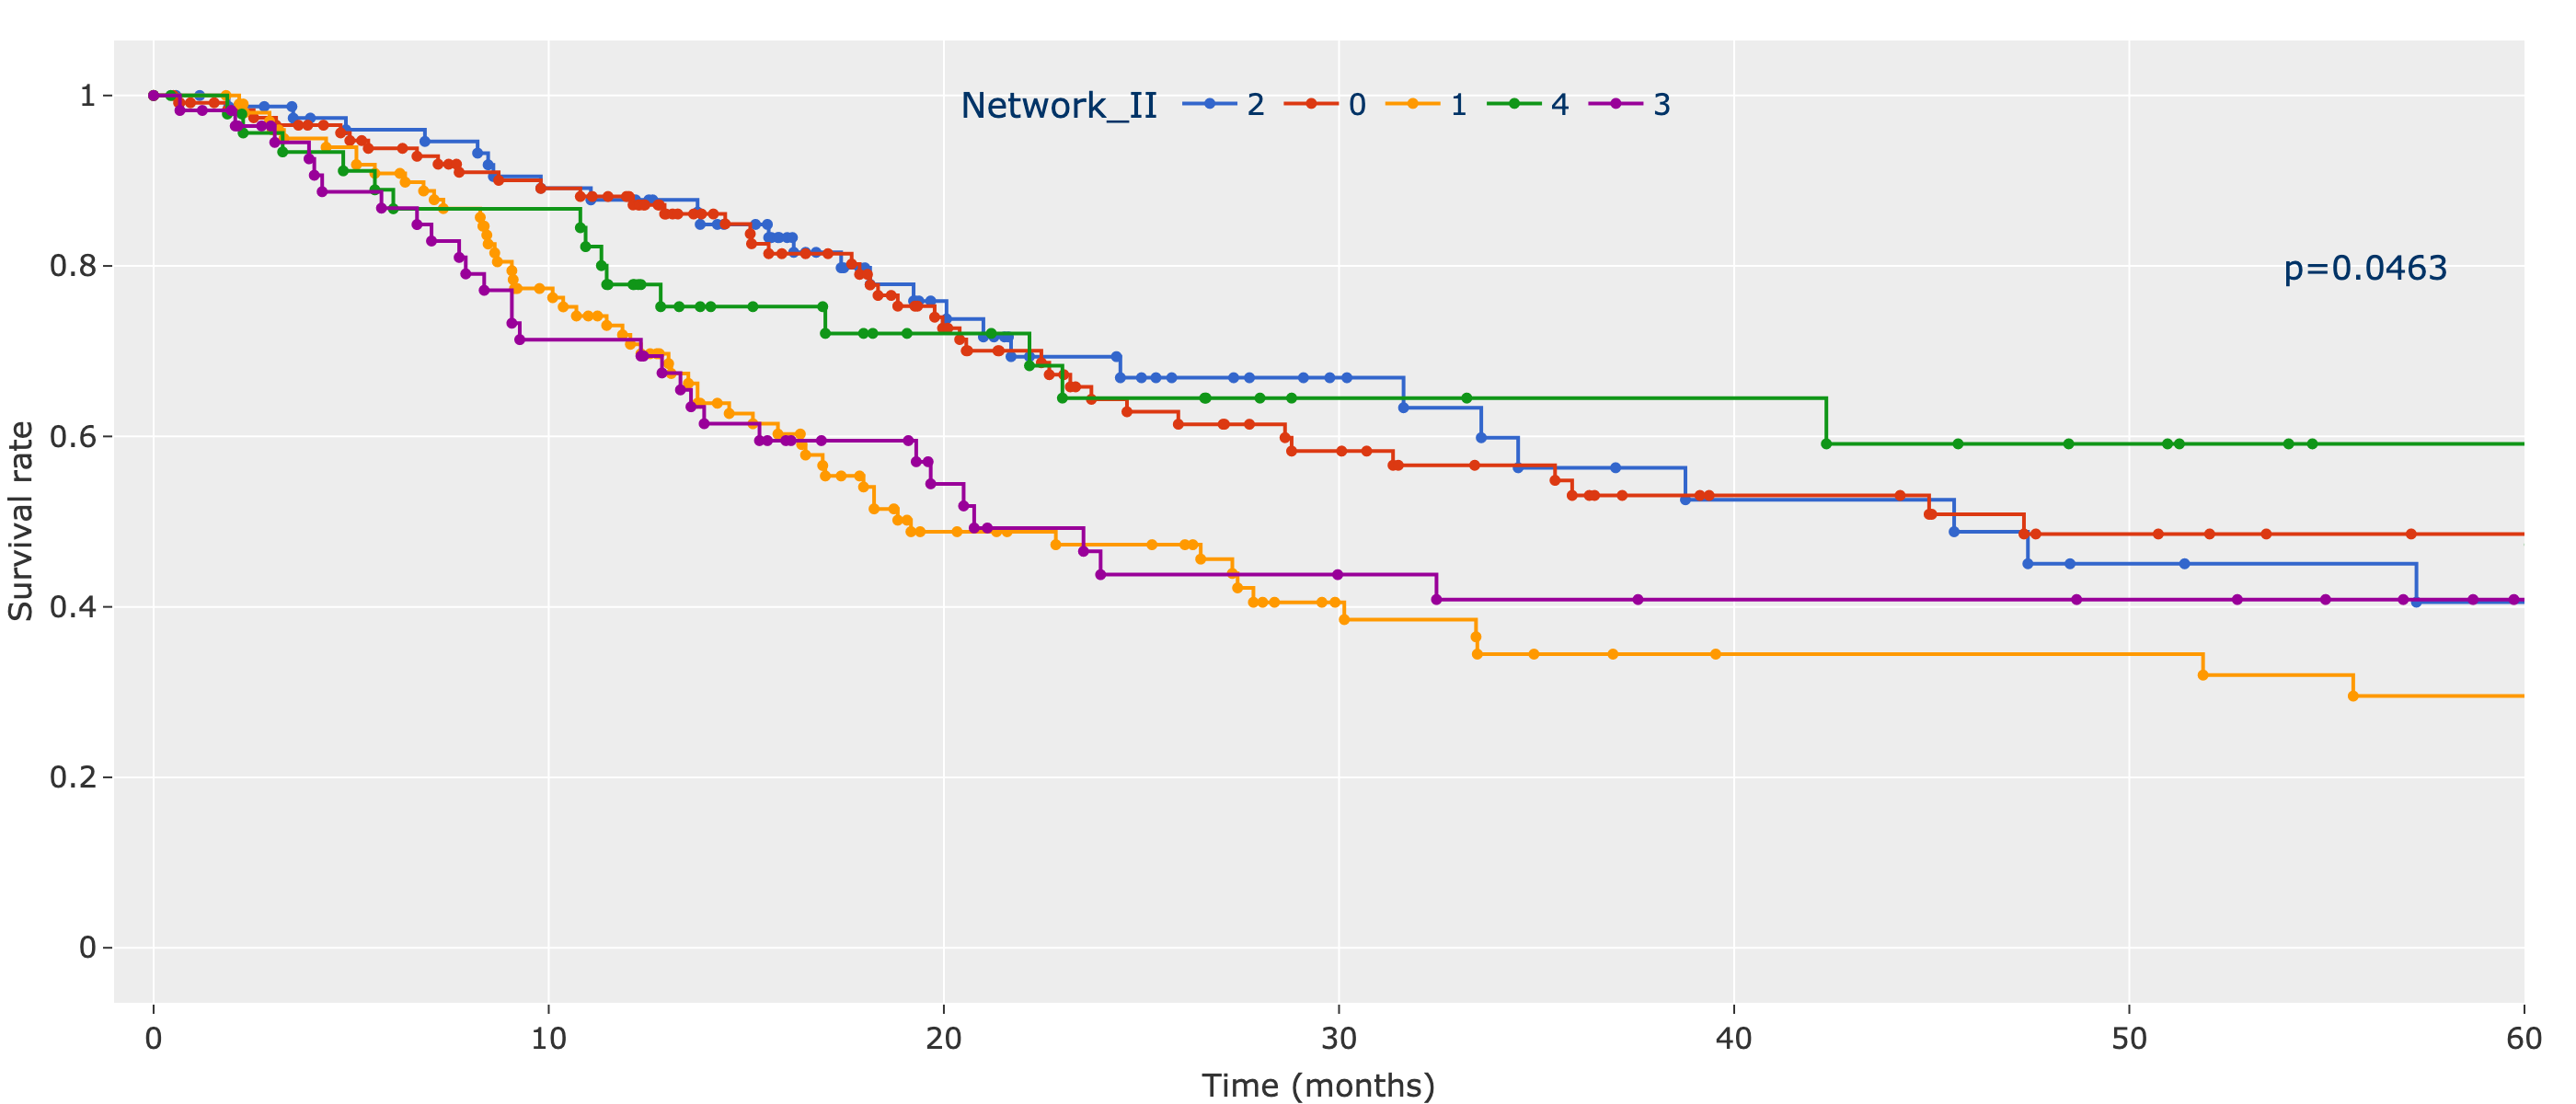
\includegraphics[width=1.0\textwidth,height=1.0\textheight,keepaspectratio]{Sections/Network_II/resources/reward/cluster_analysis/survival_K_5.png}
    \caption[Kaplan-Meier survival for when K=5 in K-means clustering]{Kaplan-Meier survival analysis of the 5 groups derived using the MEV scores (see \cref{s:N_II:rwd}) and K-means with $K=5$ (see \cref{s:ap:N_II:clustering analysis}). The plot shows the two trends in survival between the three Basal and two Luminal groups. A similar figure with $K=7$ can be seen in \cref{fig:N_II:survival_K_7}.}
    \label{fig:ap:survival_K_5}
\end{figure}

\subsection{Gene Ontology} \label{s:ap:N_II:go}


The two GO outputs represent the analysis of the 98 TFs from \cref{s:N_I:sel_tfs_go}, performed exclusively on the REACTOME database, as the HALLMARK database did not yield any notable enrichment. Details of the methodology are provided in \cref{s:lit:go}.

\begin{figure}[!htb]
    \centering
    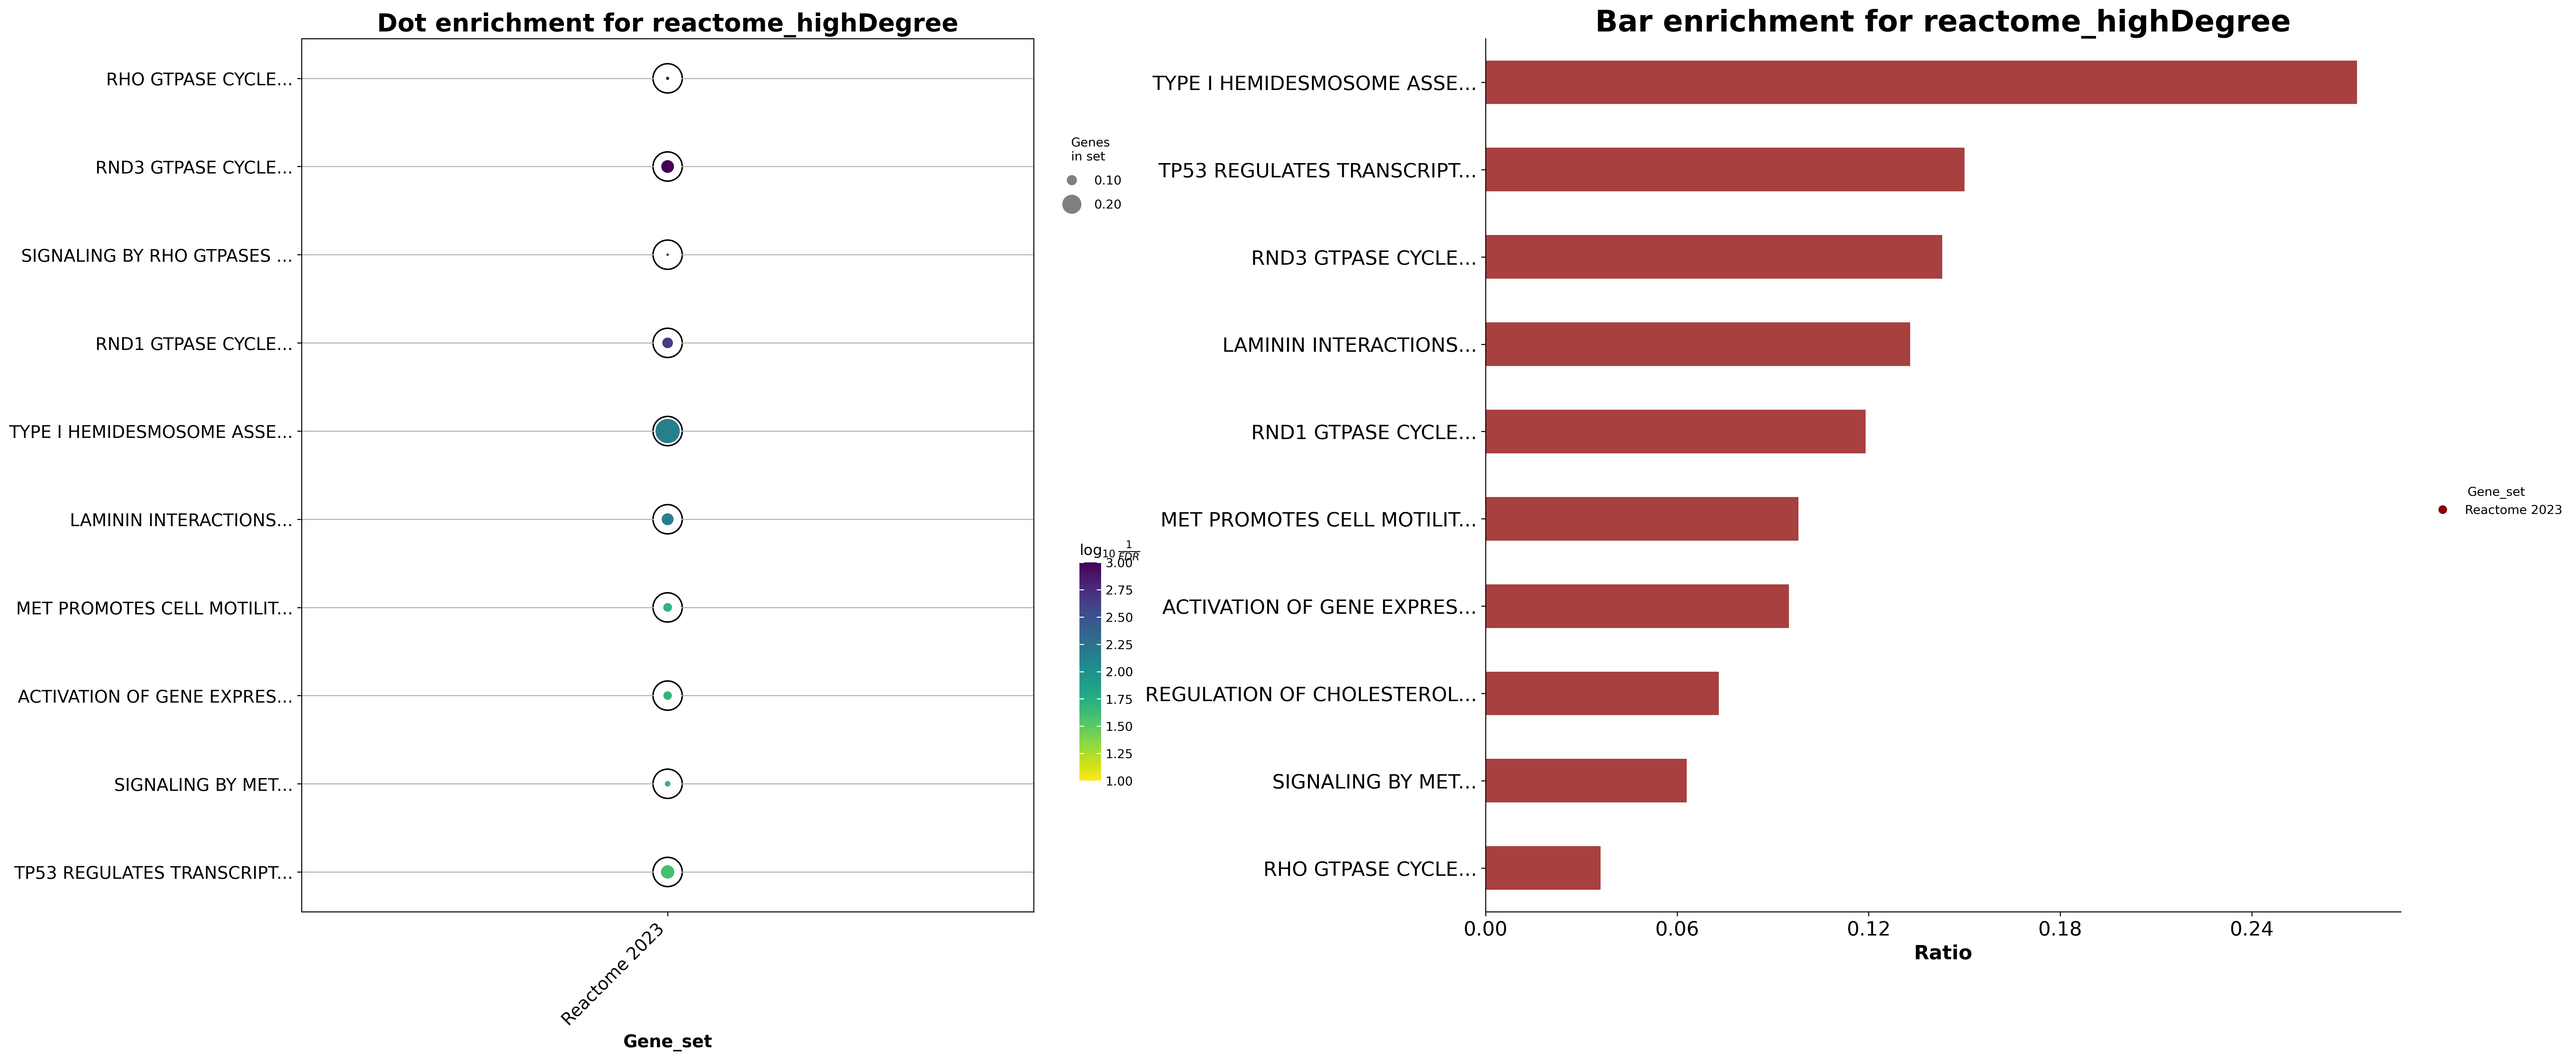
\includegraphics[width=1.0\textwidth,keepaspectratio]{Sections/Network_II/resources/reward/reactome_highDegree_dualPlot.png}
    \caption[GO analysis of the 122 genes querying REACTOME]{GO analysis of the 122 genes using the REACTOME 2023 database revealed that pathways related to epithelial structure and cell function are among the most enriched.}
    \label{fig:ap:N_II:reactome}
\end{figure}